\chapter{MORPHOLOGIE ET LEXICOLOGIE : ÉTUDES DES MORPHÈMES ET DES LEXÈMES}
\label{chapter-9}
\markright{Morphologie et lexicologie}
\origpage{239}{225}
\begin{keybox}[Plan du chapitre]
\small\setstretch{1.01}
\setlist{topsep=.12em,itemsep=.12em,parsep=0pt}
\renewcommand{\thempfootnote}{校\arabic{editorialnote}}
\textbf{I.\quad LA MORPHOLOGIE ET SES UNITÉS}
\begin{enumerate}[label=\arabic*.]
\item Notions de base de la morphologie
\begin{enumerate}[label=\textcircled{\scriptsize\arabic*}]
\item Le mot : un terme inutilisable
\item La notion de lemme
\item La notion de lexème
\item La notion de morphème
\item La notion de synthème\par
1. Définition\par 2. Exemples
\end{enumerate}
\item Les outils de la morphologie
\begin{enumerate}[label=\textcircled{\scriptsize\arabic*}]
\item Le corpus
\item L’opération de commutation
\item L’opération de permutation
\end{enumerate}
\end{enumerate}
\textbf{II.\quad TYPOLOGIE DES MORPHÈMES}
\begin{enumerate}[label=\arabic*.]
\item Morphèmes grammaticaux et morphèmes lexicaux
\item Monèmes, grammèmes et sémantèmes
\item Morphèmes libres et morphèmes liés
\item Morphèmes autonomes et dépendants
\item Morphèmes à signifiant discontinu
\item Morphèmes dérivationnels et flexionnels
\end{enumerate}
\textbf{III. LE MORPHÈME ET SES VARIANTES}
\begin{enumerate}[label=\arabic*.]
\item La notion d’allomorphe
\begin{enumerate}[label=\textcircled{\scriptsize\arabic*}]
\item Les variantes libres
\item La variantes combinatoires (contextuelles)\ednote{提纲原文 La variantes 应为 Les variantes；第227页 Les emprunt arabes 应为 Les emprunts arabes，Inférence linguistique 疑为 Interférence linguistique，与第260页正文主题相符。此处及下文均保留底本原字。}
\begin{enumerate}[label=\arabic*.]
\item L’exemple de l’imparfait en français
\item L’exemple du verbe « aller » en français
\item L’exemple d’allomorphie affixale : le préfixe privatif «/ \bipa{ɛ̃} /» en français
\item L’exemple du morphème de la pluralité en anglais
\end{enumerate}
\end{enumerate}
\origpage{240}{226}
\item Le morphème et ses difficultés de segmentation
\begin{enumerate}[label=\textcircled{\scriptsize\arabic*}]
\item Morphèmes à signifiant zéro
\item Morphèmes amalgamés
\item L’apophonie, forme de remplacement
\end{enumerate}
\end{enumerate}
\textbf{IV.\quad LA MORPHOLOGIE LEXICALE}
\begin{enumerate}[label=\arabic*.]
\item La dérivation
\begin{enumerate}[label=\textcircled{\scriptsize\arabic*}]
\item La dérivation affixale
\begin{enumerate}[label=\arabic*.]
\item Les préfixes
\item Les suffixes
\item Les infixes en grec, tagalog et bontoc et indonésien
\item Les circonfixes en allemand et indonésien
\item Les interfixes en français et allemand
\item Les suprafixes en langue ngbaka
\end{enumerate}
\item La dérivation parasynthétique
\item La dérivation impropre (conversion)\par
1. La substantivation\par
\hspace{1em}1) la métonymie\par
\hspace{1em}2) l’antonomase\par
2. L’adjectivation\par
3. L’adverbialisation
\end{enumerate}
\item La composition
\begin{enumerate}[label=\textcircled{\scriptsize\arabic*}]
\item La composition ordinaire
\item La composition savante\par
1. La place des étymos\par
2. L’allomorphie latine : les doublets\par
3. Le supplétisme\par
\hspace{1em}1) L’exemple du verbe « aller »\par
\hspace{1em}2) L’exemple de l’adjectif « ludique »\par
\hspace{1em}3) Autres exemples
\end{enumerate}
\item Siglaison et acronymisation
\begin{enumerate}[label=\textcircled{\scriptsize\arabic*}]
\item Le sigle
\item L’acronyme
\end{enumerate}
\item Troncation et métaplasmes par soustraction
\begin{enumerate}[label=\textcircled{\scriptsize\arabic*}]
\item La troncation par apocope
\item La troncation par aphérèse
\item La troncation par syncope
\item La déglutination
\end{enumerate}
\origpage{241}{227}
\item Les métaplasmes par addition
\begin{enumerate}[label=\textcircled{\scriptsize\arabic*}]
\item La prothèse
\item La paragoge
\item Le phonème éphelcystique
\item L’épenthèse
\item L’agglutination
\item La crase
\end{enumerate}
\item Les mots-valises
\begin{enumerate}[label=\textcircled{\scriptsize\arabic*}]
\item Origine du terme
\item Formation des mots-valises
\item L’haplologie
\end{enumerate}
\item L’emprunt lexical
\begin{enumerate}[label=\textcircled{\scriptsize\arabic*}]
\item Les raisons de l’emprunt lexical
\item Inférence linguistique et emprunts lexicaux\par
1. L’adstrat italien\par 2. Les emprunt arabes
\item Les adaptations dans la langue d’arrivée\par
1. Adaptations phonologiques\par 2. Adaptations grammaticales\par
3. Doublement des pluralisations\par 4. Les doublets germaniques et romans
\item Emprunts et réemprunts : l’exemple anglais
\end{enumerate}
\end{enumerate}
\textbf{Exercices}\par
\textbf{Pour aller plus loin}\par
\textbf{Glossaire}
\end{keybox}

\origpage{242}{228}
\begin{keybox}[Introduction]
\renewcommand{\thempfootnote}{校\arabic{editorialnote}}
Dans le chapitre 4, nous avons vu qu’utiliser le vocabulaire courant en logique ou en philosophie est problématique, et c’est la même chose en linguistique. Ainsi, lorsque l’on veut, avec nos mots, définir la notion de « mot », plusieurs problèmes se posent, un peu comme si un grain de sable voulait expliquer le désert. D’où la nécessité d’avoir recours au métalangage, langage formel conçu spécifiquement pour décrire rigoureusement le langage.

Dans une première approche, on peut bien sûr dire qu’un mot est une suite de sons ou de caractères graphiques formant une unité sémantique et pouvant être distingués par un séparateur (un blanc typographique). Mais cette définition connaît des limitations : certaines écritures n’utilisent pas le blanc typographique : c’est le cas du chinois, où rien n’indique dans l’écriture les limites entre les « mots ». Par ailleurs, la grande majorité des langues ne sont pas écrites, et le blanc typographique ne peut s’entendre à l’oral. Une personne écoutant un énoncé dans une langue qu’elle ne connaît pas ne pourra pas en identifier les mots. Elle entendra des sons, et si elle sait ce qu’est un phonème, elle pourra éventuellement les identifier, mais sans comprendre le sens de l’énoncé.

D’un point de vue plus pratique à présent, est-il logique que « ceci » compte pour un mot, et que « ceux-ci » compte pour deux mots alors que phonologiquement ils sont identiques et ne diffèrent que par un trait d’union ?\ednote{ceci 与 ceux-ci 并非音系形式相同：通常分别为 \bipa{/səsi/} 与 \bipa{/søsi/}。二者也不只相差连字符；ceux-ci 在通常法语正字法中视为连字符复合代词，不宜不加说明便算作“两词”。例词仍依原书保留。} De même, que penser d’« aujourd’hui » ou des prépositions et articles contractés « du », « aux », « des » : comptent-elles pour un mot ou deux mots ? Dernier exemple enfin : « pomme de terre », « fer à repasser » comptent-ils pour un ou trois mots ? Dans ce chapitre, nous allons faire nos adieux au « mot » et le remplacer par des notions plus adaptées à la description linguistique.
\end{keybox}

\section{LA MORPHOLOGIE ET SES UNITÉS}
Étymologiquement, la morphologie, est « la science des formes ». En linguistique, ce terme s’emploie pour désigner l’étude des formes sous lesquelles se présentent les mots dans une langue donnée. Située entre la phonologie et la syntaxe, qui est étude de la combinaison des mots, son objet est étude de la structure interne des mots. Dans son très célèbre ouvrage \textit{Language}, le grand linguiste et anthropologue américain \textbf{Leonard Bloomfield} (1887-1949)\origfoot{1}{Nous retrouverons Leonard Bloomfield, considéré par certains comme « le Saussure français », dans le chapitre 14, consacré au structuralisme américain.}\ednote{原注称 Bloomfield 为 « le Saussure français »，与正文所述 américain 及其美国结构主义背景不合，此处 français 疑应为 américain；“被某些人如此称呼”的具体出处未注明，不据此另造引文。本段 qui est étude 和 son objet est étude 均缺冠词 l’。} la définit ainsi :
\begin{quote}\small\itshape
Nous pouvons dire que la morphologie comprend les constructions des mots ou des parties de mots, tandis que la syntaxe comprend les constructions de syntagmes.
\end{quote}

\origpage{243}{229}
\subsection{Notions de base de la morphologie}
Pour les linguistes, il est nécessaire de supprimer le terme de « mot » de leur vocabulaire. Après avoir expliqué d’où vient cette nécessité, nous verrons que, pour le remplacer, avons l’embarras du choix : « lemme », « item lexical », « lexie » ou encore « unité lexicale ».\ednote{pour le remplacer, avons 缺少主语 nous。另，“所有语言学家必须取消 mot”是作者的立场，不是全学科统一术语规范；本章后文实际仍使用 mot。词、词位、词目形式与语素各有分析用途，参见\ecite{49}。}

\minititle{\textcircled{\scriptsize 1} Le mot : un terme inutilisable}
Dans les exemples ci-dessous, nous allons voir les notions de forme et d’occurrence pour, dans un premier temps, limiter un peu l’imprécision du terme « mot ».

\noindent\textbf{Ex. 1 : Le} livre de linguistique est dans \textbf{le} tiroir.

Dans cet exemple, certains personnes comptent six mots, d’autres cinq en comptant comme un seul mot les deux fois où « le » apparaît. On voit que l’on peut faire une distinction entre ce que l’on lit ou entend physiquement (les occurrences) et les unités formelles (les formes) qui peuvent apparaître plus d’une fois. Ainsi, dans ce premier exemple, on dira qu’il y a six occurrences, et que deux d’entre elles sont des occurrences de la forme « le ».\ednote{按原例逐词计数：Le / livre / de / linguistique / est / dans / le / tiroir，共8个词次；忽略句首大小写后为7种词形，并非6与5。certains personnes 应为 certaines personnes。}

\noindent\textbf{Ex. 2 : Un grand} homme avec \textbf{une grande} ambition.

Ici, la situation se complique un peu. Certains locuteurs diront qu’il y a sept mots, tandis que d’autres n’en verront que cinq. Les premiers comptent les occurrences, tandis que les autres comptent ensemble « un » / « une » et « petit » / « petite ». On voit que l’on peut faire une deuxième distinction et analyser certaines formes comme les manifestations d’une même occurrence. Ainsi, l’adjectif « petit » possède quatre formes possibles à l’écrit (« petit », « petits », « petite », « petites ») et deux formes à l’oral : \bipa{[p(ə)ti], [p(ə)tit]}. Chacune de ces formes peut avoir une ou plusieurs occurrences dans un texte.\ednote{本例使用的是 grand / grande，说明中的 petit / petite 与例句不符；可相应改为 grand / grande，或把例句中的形容词改为 petit / petite，但正文不作替换。“同一 occurrence 的不同形式”也混淆层级，此处应指同一词位或词汇单位，而非同一次出现。}

\noindent\textbf{Ex. 3 :} Je \textbf{lis} le livre de linguistique que tu \textbf{lisais} hier.

On note ici la présence de deux formes distinctes d’un même verbe. Il y a donc huit occurrences et huit formes (ou seulement sept si l’on regroupe « lis » et « lisais »).\ednote{按印出的例句，Je / lis / le / livre / de / linguistique / que / tu / lisais / hier，共10个词次及10种词形；把 lis 与 lisais 归并为同一词位后为9个单位，不是8、8、7。}

\noindent\textbf{Ex. 4 :} Je \textbf{lirai} le livre que tu \textbf{as lu} hier.

L’exemple 4 ajoute encore une complication. Faut-il traiter comme une seule forme « as lu » ? Pour justifier un tel choix, on pourra justifier que « as lu » n’est qu’une seule forme (le passé composé) du verbe « lire ». Pour justifier le contraire, on pourra signaler qu’il est possible de séparer « as » de « lu ». Par exemple, dans « tu n’as pas lu le livre ».

\noindent\textbf{Ex. 5 :} Je \textbf{la} vois : elle est derrière \textbf{la} maison rouge.

L’exemple 5 ajoute une autre complication. On trouve deux occurrences d’une même forme (« la »), mais s’agit-il vraiment de la même forme ? La première occurrence est un article, la seconde un pronom. Même forme, donc, mais des fonctions différentes. Difficile de trancher.\ednote{两处词类颠倒：Je la vois 中第一个 la 是宾语代词；la maison 中第二个 la 是定冠词。}

\noindent\textbf{Ex. 6 :} Je \textbf{bois} de l’eau, dans un \textbf{bois}, assis sur une chaise en \textbf{bois}.

\origpage{244}{230}
Dans l’exemple 6, on trouve trois occurrences de « bois ». La première occurrence est un verbe, les deux autres sont des substantifs homophones. Certains linguistes y verront deux mots distincts, d’autres n’y verront qu’un seul.

Face à ce casse-tête, les linguistes ont abandonné la notion de « mot » au profit de terminologies plus scientifiques et plus précises. Voici comment \textbf{André Martinet}, père de l’analyse fonctionnaliste en linguistique française, justifie son abandon :
\begin{quote}\small\itshape
Puisqu’il n’y a pas moyen de définir simplement le terme « mot » de façon à faire concorder cette définition avec l’usage ordinaire que l’on en fait, les structuralistes font de ce terme un usage aussi restreint que possible.

Notre conclusion est, évidemment, que ce terme de « mot » est inutilisable, aussi bien dans une recherche syntaxique sérieuse que dans la présentation de ses résultats.
\end{quote}
Une fois le « mot » abandonné, par quoi le remplace-t-on ? Nous avons l’embarras du choix.

\minititle{\textcircled{\scriptsize 2} La notion de lemme}
En morphologie, l’unité autonome constituante du lexique d’une langue est appelée « lemme ». Dans les langues indo-européennes, le lemme est une unité de sens et de son, il est constitué de morphèmes, eux-mêmes constitués de phonèmes : c’est la fameuse double articulation du langage que l’on doit à André Martinet. Prenons l’exemple du lemme le plus long en français : « anticonstitutionnellement ». Il possède 19 phonèmes (\bipa{[ɑ̃tikɔ̃stitysjɔnɛl(ə)mɑ̃]}) et 6 morphèmes : « anti- », « con- », « -stitu- », « -tion », « -nelle », « -ment ».\ednote{本段采用的 lemme、lexème 用法不等同于许多形态学及词典学著作的约定：常以 lexème 指抽象词汇单位，lemme 指其词典代表形式，不能一概把 lexème 等同于词根。参见\ecite{49}。所列音标按括号内 schwa 实现与否分别为19或18个音段，计数需说明；其6段切分混合了不同历史层次，不能仅由拼写证明各段在共时分析中均为独立语素。}

Dans les langues isolantes, les lemmes ne sont pas composés de morphèmes, car les signes ne sont pas décomposables. Ainsi, en mandarin, 心 est à la fois un caractère (字) et un lemme (词). Mais il existe aussi dans ces langues des « lemmes composés » (合成词) comme 大学, composé des deux lemmes 大 et 学. La « pomme de terre » évoquée dans l’introduction est elle aussi un lemme composé.\ednote{单语素词仍由一个语素构成，不能说“不由语素构成”；孤立型也不排除复合构词，原段自己的大学例已说明这一点。文字单位“字”与语法单位“语素／词”应分别判断，不能从是否可分解字形直接推出语素结构。}

\minititle{\textcircled{\scriptsize 3} La notion de lexème}
Le lexème, appelé aussi « unité lexicale », désigne le morphème lexical d’un lemme. Dans « cet étudiant est remarquable », « remarqu- » est le lexème du lemme « remarquable ».

Le lexème est souvent assimilé au radical du lemme : dans toutes les formes de conjugaison d’un verbe, on retrouve le même lexème. Ainsi, les formes « aimer », « aime », « aimé », « aimions » ou « aimât », etc, sont les formes fléchies d’un même lexème : aim-. On parle dans ce cas d’un lexème « lié », car il n’existe pas de forme libre du lexème aim- : il est obligatoirement suivi d’un morphème flexionnel. Inversement, il existe des lexèmes libres comme « choix », « sol », « livre », qui ne se rencontrent que sous une seule forme. C’est pour cela que les lemmes qui ne sont composés que d’un seul lexème ( « femme », « maison », « demain », etc.) sont parfois appelé « lexèmes » par certains linguistes : « table », par exemple, est à la fois un lemme, un lexème, et un
\origcont{245}{231}morphème.

\minititle{\textcircled{\scriptsize 4} La notion de morphème}
On l’a vu : le lemme est une unité sémantique, elle-même composée d’unités de sens non décomposables, les morphèmes. Dans le lemme « immangeable », il y a trois morphèmes « -in », « -mange- », « -able », et chaque morphème porte un sens. Notez au passage que le morphème « -mange- », est un lexème. Autre exemple, le lemme « lecteurs » est composé de trois morphèmes :
\begin{itemize}
\item « lect- » : lexème, action de lire
\item « -eur- » : celui qui fait
\item « -s » : marque du pluriel
\end{itemize}
On voit ici que « s » peut-être un phonème, mais aussi un morphème remplissant une fonction grammaticale.\ednote{本例的复数拼写 -s 通常不发音，不能把字母 s、音位 /s/ 和复数语素直接等同。可改为“书写上的 -s 标示复数，而其语音实现须另行分析”。peut-être 在此应为 peut être；上文前缀 -in 的连字符位置应为 in-，immangeable 中的拼写变体为 im-。}

\minititle{\textcircled{\scriptsize 5} La notion de synthème}
Revenons à présent à notre « pomme de terre ». Originellement composé de trois morphèmes distincts, ce lemme composé s’est lexicalisé. Aujourd’hui, il est considéré comme un seul morphème (lemme), indécomposable et doté d’une unité sémantique. Pour André Martinet, c’est un « synthème ».\ednote{“词汇化后等于一个不可分语素”与紧接着所引 Martinet 定义不一致：引文明确要求可分析为两个或更多 monèmes。作为一个句法单位运作，不等于内部不再具有语素结构；应区分功能上的整体性与内部可分析性。}

\minititle{1. Définition}
André Martinet définit ainsi le synthème :
\begin{quote}\small\itshape
Un synthème est une unité significative, formellement et sémantiquement analysable en deux ou plus de deux monèmes, mais qui, syntaxiquement, entretient les mêmes relations avec les autres éléments de l’énoncé que les monèmes avec lesquels il alterne.
\end{quote}
Pour ne pas gêner la compréhension, je m’empresse de préciser que pour Martinet le « monème » correspond à ce que nous appelons de nos jours un morphème. Nous reviendrons sur ce terme de monème un peu plus tard. Dans l’immédiat, retenez qu’un synthème est une combinaison figée de morphèmes qui fonctionne comme un seul morphème et qui, malgré son caractère composite, appartient à une classe de morphèmes.

\minititle{2. Exemples}
Parmi les exemples de syntagmes, on peut citer :
\begin{itemize}
\item les dérivés diminutifs : « maisonnette », « fillette », « chansonnette », « biquet », « cochonnet », etc. Ces unités significatives sont formées d’un lexème et d’un morphème de signifié « petit ».
\item les adjectifs composés, comme « indésirable », « incompréhensible », « faisable », «irritable», etc. Ils combinent un lexème (verbal) et un morphème de signifiant /abl/ de signifié « qui peut \origcont{246}{232}être ». Les deux premiers exemples ajoutent un troisième morphème de signifiant / \bipa{ɛ̃} / (« in- ») et de signifié « pas ». Ces syntagmes de radical verbal appartiennent à la classe de morphèmes des adjectifs.\ednote{incompréhensible 的后缀为 -ible（\bipa{/ibl/}），不能把四例一概记为 /abl/。这些形容词按本章后文的分类属于派生词，不宜与独立词汇单位组合的 composition 混同；本段 syntagmes 与 synthèmes 的用词也需区分。}
\item les mots composés : « tire-bouchon », « taille-crayon », « lave-vaisselle », « sèche-cheveux », etc. Ils combinent un verbe et un nom pour former un synthème, qui, au final est un nom. Les synthèmes de type « machine à laver », « machine à écrire », « table à repasser », « fer à repasser », « mousse à raser » qui combinent un nom, un morphème de signifiant discontinu (/à ... infinitif/) de signifié « pour » (nous y reviendrons un peu plus bas), et un lexème verbal, forment une unité syntaxique et sémantique minimale qui appartient à la classe des noms.
\end{itemize}
Dans la mesure où ils sont l’équivalent \textit{fonctionnel} d’un morphème unique, les synthèmes ont vocation à devenir des unités significatives minimales, c’est-à-dire des morphèmes libres (lemmes). C’est la raison pour laquelle des lemmes composés comme « pomme de terre » ou « fourchette » sont maintenant non analysables en unités significatives plus petites, alors qu’ils étaient, lors de leur création, d’authentiques synthèmes, c’est-à-dire des combinaisons de morphèmes. En effet, la pomme de terre était un « fruit de la terre », et la « fourchette », une « petite fourche ». Pour un locuteur français actuel, « pomme de terre » s’oppose globalement à « carotte » ou « tomate », et pas « *pomme de mer » ou « *poire de terre ». De même, « fourchette » s’oppose à « cuillère » ou « couteau ». Ces synthèmes sont devenus des lexèmes aussi indécomposables que les lexèmes auxquels ils s’opposent (« tomate » ou « cuillère »).

\subsection{Les outils de la morphologie}
Dans le chapitre précédent, on voit que les outils du Cercle Linguistique de Prague sont si rigoureux et efficaces qu’ils ont réutilisés dans d’autres domaines de la linguistique.\ednote{ont réutilisés 缺少 été，应为 ont été réutilisés。} Et en effet, depuis le structuralisme, les linguistes utilisent beaucoup la procédure de la commutation pour justifier leurs analyses. L’analyse morphologique, comme l’analyse phonologique, repose sur un corpus et sur l’opération de commutation, mais aussi sur une opération qui lui est spécifique : la permutation.

\minititle{\textcircled{\scriptsize 1} Le corpus}
L’analyse morphologique procède à partir d’un corpus, échantillon représentatif de données linguistiques sélectionnées et organisées en vue de l’analyse linguistique. Il peut être présenté sous forme graphique, mais en raison du principe de la primauté accordée à l’oral, on privilégie en général la transcription phonétique ou phonologique. Dans les très nombreuses langues dépourvues de système d’écriture, la transcription du corpus est la seule manière de procéder.

\minititle{\textcircled{\scriptsize 2} L’opération de commutation}
On utilise deux tests différents en morphologie. Le premier, que nous connaissons, est le test de commutation. Dans ce test, on essaie de trouver quels éléments (morphèmes) sont susceptibles de prendre la place d’un autre phonème. Le résultat obtenu est un paradigme, c’est-à-dire un ensemble de phonèmes qui pourraient remplacer le phonème faisant l’objet de la commutation.\ednote{此处研究的是 mon / ton / leur 以及 professeur / ami 等语法或词汇单位的替换，连续出现的 phonème(s) 应按所分析层级改为 morphème(s) 或 unité(s)，不能把后文所列词当作音位。} Ceci devrait vous rappeler les rapports paradigmatiques de Saussure. Par exemple, si l’on fait \origcont{247}{233}un test de commutation sur « mon » dans « mon professeur de français », on obtiendra une liste comprenant « mon », « ton », « leur », « notre », « votre », « le », « un », « ce », etc. Même chose si la commutation porte sur « professeur », où l’on obtiendra le paradigme « ami », « drapeau », « dictionnaire », « fromage », etc.

\minititle{\textcircled{\scriptsize 3} L’opération de permutation}
Le test permutation, spécifique, on l’a dit, à la morphologie, consiste à changer l’ordre des lemmes pour voir quels lemmes peuvent se placer dans quelles positions. Ici, le résultat obtenu n’est pas un paradigme, mais un syntagme.\ednote{Le test permutation 应为 Le test de permutation。以整词或副词在句中的位置变换为例，涉及的是句法分布；不能称置换测试专属于形态学。}

Par exemple, on peut dire indifféremment :
\begin{quote}
\textbf{Ex :} J’ai étudié la linguistique hier.

\hspace{1.8em}Hier, j’ai étudié la linguistique.
\end{quote}
Mais, on ne peut pas dire :
\begin{quote}
\textbf{Ex :} *J’ai hier étudié la linguistique.
\end{quote}
Nous verrons un petit peu plus bas que c’est précisément ce test de permutation qui permet de valider les deux formes « je puis » et « puis-je » et d’invalider la forme « *peux-je ».

\section{TYPOLOGIE DES MORPHÈMES}
On peut dire qu’il existe deux grandes catégories de morphèmes : les morphèmes lexicaux et les morphèmes grammaticaux.

\Needspace{5\baselineskip}
\subsection{Morphèmes grammaticaux et morphèmes lexicaux}
Martinet définit les morphèmes lexicaux (lexèmes) comme des morphèmes qui appartiennent à des inventaires illimités. Les morphèmes grammaticaux, quant à eux, sont des morphèmes qui font partie de paradigmes dont les membres sont en nombre réduit :
\begin{quote}\small\itshape
Les monèmes lexicaux sont ceux qui appartiennent à des inventaires illimités. Les monèmes grammaticaux sont ceux qui alternent dans les positions considérées, avec un nombre relativement réduit d’autres monèmes. La fréquence des monèmes grammaticaux est bien supérieure à celle des monèmes lexicaux.
\end{quote}
\begin{itemize}
\item Les morphèmes grammaticaux sont en nombre limité et appartiennent à une classe fermée. Ce sont les pronoms, les prépositions, les conjonctions, les déterminants, les affixes, les désinences (pluriel, féminin, et terminaisons verbales). Les morphèmes grammaticaux ont la double caractéristique de ne jamais varier et de ne pas voir leur nombre augmenter. En français, nous disposons par exemple de trois formes d’articles définis, « le », « la », « les » : on imagine mal les hommes inventer un quatrième déterminant.\ednote{“封闭类”不意味着形式永不变化、历史上永不增加；本章随后讨论语法语素的异形态，已与 ne jamais varier 的绝对说法不符。定冠词类也不等于全部限定词类，应将 quatrième déterminant 限定为第四个定冠词成员。}
\origpage{248}{234}
\item Les morphèmes lexicaux (lexèmes), quant à eux, appartiennent à une classe ouverte qui comprend les noms, les adjectifs, les verbes et adverbes : cette liste évolue, avec des créations (par exemple, « \textit{duang !} » en chinois) et mais aussi disparitions.\ednote{et mais aussi disparitions 应为 mais aussi des disparitions，或 et aussi des disparitions。}
\end{itemize}

\subsection{Monèmes, grammèmes et sémantèmes}
Dans la terminologie de la linguistique fonctionnelle d’André Martinet, les morphèmes grammaticaux et lexicaux définis ci-dessus sont regroupés sous le terme unique de « monèmes ».
\begin{itemize}
\item Le morphème lexical est appelé « sémantème ». Martinet nous donne un exemple d’utilisation de sa terminologie : « travaillons » comporte deux morphèmes, chacun porteur de sens :
\begin{quote}
- un sémantème : « travail- »

- un morphème : « -ons »
\end{quote}
Dans la terminologie actuelle, on parle plutôt de « lexème », le terme de « sémantème » étant de nos jours utilisé en sémantique\origfoot{2}{Nous verrons cela dans le chapitre 11, dans la partie consacrée à la sémantique componentielle de Bernard Pottier.}.
\item Le « grammème » est l’équivalent du morphème grammatical. Par exemple, le lemme « tristement » se décompose en deux monèmes :
\begin{quote}
- « triste- » : sémantème (lexème)

- « -ment » : grammème.
\end{quote}
\end{itemize}
Martinet a développé les entités abstraites que sont les monèmes pour rendre compte de sa célèbre notion de double articulation des unités constitutives de la langue. Les monèmes sont les unités de première articulation, les phonèmes sont les unités de seconde articulation. Répétons toutefois que les termes de monème et de grammème ne sont plus guère usités de nos jours : on leur préfère les termes de morphème lexical ou grammatical.

\subsection{Morphèmes libres et morphèmes liés}
Nous avons vu un peu plus haut que les lexèmes peuvent être « libres » ou « liés ». De la même manière, un morphème est libre s’il peut constituer un lemme à lui tout seul. Par exemple, « le », « livre », « de », « linguistique » sont tous des morphèmes libres. À l’opposé, un morphème est lié s’il n’existe jamais à l’état libre et doit être rattaché à un autre morphème. Par exemple, la flexion « -ons » dans « mangeons », le préfixe « re- » dans « recommencer » sont deux morphèmes liés.

\subsection{Morphèmes autonomes et dépendants}
On peut dire d’un morphème qu’il est autonome s’il peut constituer non pas un lemme mais un \textit{énoncé} à lui tout seul, comme une réponse à une question, et ne dépend pas d’autres éléments. Par exemple si l’on vous demande : « Comment trouvez-vous ce chapitre sur la morphologie », il y a fort à parier que \origcont{249}{235}beaucoup d’entre vous répondront : « difficile », « ennuyeux », « mortel », « terrible », « déprimant », etc. Bien sûr, vous ne serez pas à court de morphèmes autonomes pour vous exprimer ! Mais faites votre attention sur un point : même s’il est \textit{libre} d’un point de vue formel, un morphème peut être \textit{dépendant} lorsqu’il ne peut qu’apparaître accompagné d’autres unités lexicales ou s’il est lié, même de façon implicite, à d’autres unités lexicales. Prenons quelques exemples :
\begin{itemize}
\item Le morphème grammatical « il » est libre mais dépendant, et pour deux raisons. D’abord, il ne peut constituer un énoncé indépendant : on ne peut répondre à une question par « il ». Ensuite, il faut savoir que l’on utilise les pronoms personnels pour ne pas répéter un antécédent déjà évoqué, comme dans « \textit{Mon professeur} est vraiment gentil : \textit{il} m’a offert son livre de linguistique ». Dans cet énoncé, le morphème « il » entretient un lien avec « mon professeur » (son antécédent) : il est donc dépendant.
\item Si au moment de commander un café, le serveur me demande : « avec ou sans sucre ? », je peux me contenter de répondre « avec », mais « avec » ne peut à lui seul constituer un énoncé valide, car il \textit{sous-entend} un autre terme : le référent « sucre », que je n’ai pas répété en raison du contexte de la conversation déjà connu de moi et du serveur. « Avec » est donc, lui aussi, un morphème dépendant.
\item Si l’on vous demande « quand retourneras-tu à la bibliothèque », vous pouvez répondre « demain », qui est un morphème dépendant. En effet, dans une situation de communication, « demain » sous-entend toujours « demain \textit{par rapport au moment où je parle}. »
\end{itemize}
En linguistique de l’énonciation\origfoot{3}{Embrayeurs, déictiques et anaphores seront présentés en détail dans le chapitre 12, dans la partie consacrée à la linguistique de l’énonciation.}, ces pronoms et compléments circonstanciels de temps sont appelés « embrayeurs » ou « déictiques ».\ednote{辨析：这里混用了句法依附、照应关系和语境指示三个标准。demain 的解释依赖说话时间，不因此便在句法上依附于另一个词；上文“difficile”作为简短回答也依赖问题语境。故语境依赖本身不足以划分所谓自主与依附语素。}

\subsection{Morphèmes à signifiant discontinu}
Nous avons vu tout à l’heure que les synthèmes « fer à repasser » ou « machine à écrire » contiennent un morphème « à signifiant discontinu ». Pour employer la terminologie morphologique, on parle de morphème à signifiant discontinu lorsqu’\textit{un seul signifié} peut être associé à deux segments phoniques non contigus (autrement dit, séparés) dans la chaîne parlée. Comme cela semble un peu compliqué, passons directement aux exemples. Pour illustrer les morphèmes à signifiant discontinu, prenons l’exemple utilisé par André Martinet lui-même :
\begin{quote}\textbf{Ex :} Nous courons.\end{quote}
Dans l’énoncé \bipa{/nukuRɔ̃/}, Martinet considère que « nous » (/nu/) et « -ons » (\bipa{/ɔ̃/}) représentent un seul signifiant : le signifiant discontinu du signifié « première personne de pluriel ». En effet, si l’on applique le test de commutation, et si nous choisissons la 2\textsuperscript{e} ou la 3\textsuperscript{e} personne du pluriel à la place de la 1\textsuperscript{re} personne, alors nous devrons remplacer non seulement /nu/, mais aussi \bipa{/ɔ̃/}, pour obtenir « vous courez » ou « ils courent », et non pas « *vous courons » ou « *ils courons », ni non plus « *nous courez », \origcont{250}{236}si par exemple on ne remplaçait que la désinence \bipa{/ɔ̃/}. Le signifiant que l’on doit associer au signifié « personne du pluriel » est donc l’ensemble des \textit{deux} segments phoniques non contigus « nous » /nu/ et « -ons » \bipa{/ɔ̃/}. On dira donc que \bipa{/nu...ɔ̃/} est le signifiant d’un morphème unique et constitue une unité significative minimale. Autre exemple en français : le morphème de la négation « ne...pas » est lui aussi un morphème discontinu.

\subsection{Morphèmes dérivationnels et flexionnels}
Les morphèmes dérivationnels (affixes) servent à la création de nouveaux mots lexicaux par une opération appelée « dérivation ». On peut distinguer deux types principaux de morphèmes dérivationnels selon deux critères :
\begin{itemize}
\item La place qu’ils occupent par rapport à la base lexicale (lexème) sur laquelle ils se greffent : devant (préfixe), derrière (suffixe), à l’intérieur (infixe), à travers (transfixe), de chaque côté de la base (circonfixe), au dessus (circonfixe).\ednote{末尾 au dessus (circonfixe) 与前项重复，按后文第243页应为 suprafixe，即通过声调、重音等超音段特征实现的词缀；并非又一种环缀。}
\item Leur effet sur la catégorie de la base sur laquelle ils se greffent : par exemple transformation par affixe (ici, préfixe) d’un verbe en adjectif (« lire » $\rightarrow$ « lisible »), ou d’un adjectif en adverbe (« rapide » $\rightarrow$ « rapidement »).\ednote{两例都不涉及前缀，应将 ici, préfixe 改为 ici, suffixe：-ible 与 -ment 位于词基之后。}
\end{itemize}
Les morphèmes flexionnels (flexions), quant à eux, indiquent la relation que le radical verbal (lexème) auquel ils s’ajoutent entretient avec les autres unités de l’énoncé. On distingue deux types principaux de flexions selon la catégorie de la base :
\begin{itemize}
\item Les flexions nominales, adjectivales et pronominales. Elles sont de deux sortes en français : le genre, et le nombre. « cheval$\rightarrow$chevaux », « heureux$\rightarrow$heureuse », « il$\rightarrow$ils », etc. sont des exemples de flexion nominale, adjectivale et pronominale.
\item Les flexions verbales. Elles correspondent en français à la conjugaison des verbes, véritable cauchemar pour tous les étudiants en français. Elles ont pour fonction de marquer la personne, le nombre, le temps, le mode et la voix (actif ou passif).
\end{itemize}
Notons que le morphème flexionnel ne modifie jamais la catégorie de la base à laquelle il s’adjoint, contrairement aux morphèmes dérivationnel.\ednote{dérivationnel 应为 dérivationnels；派生词缀也并不总改变词类，如本章自己的 recommencer 仍是动词。因此“与派生相反”不能理解为所有派生都改变词类。}

\section{LE MORPHÈME ET SES VARIANTES}
Dans le chapitre précédent, nous avons vu que le même phonème peut se manifester sous plusieurs formes différentes, sans que cela change le sens : ce sont des allophones. Un morphème peut lui aussi prendre plusieurs formes selon des contextes phonologiques ou morphologiques différents.

\subsection{La notion d’allomorphe}
Comme en phonologie, on distingue deux sortes de variantes : les variantes libres, qui sont
\origcont{251}{237}indépendantes du contexte d’apparition du morphème, et les variantes combinatoires (contextuelles), qui sont entraînées par le contexte d’apparition du morphème.

\minititle{\textcircled{\scriptsize 1} Les variantes libres}
Certains morphèmes peuvent présenter des variations en dehors de toute nécessité contextuelle. Ainsi, en français, on dit « je peux » \bipa{[ʒə pø]}, ou « je puis » \bipa{[ʒə pyi]} : le locuteur est libre de choisir l’une des deux formes. Mais cette liberté a une limite : l’opération de permutation (vue plus haut) nous indique que l’inversion du pronom personnel entraîne obligatoirement l’allomorphe \bipa{[pyi]}. Ainsi, « que puis-je faire ? » est correct, « *que peux-je faire ? » ne l’est pas.\ednote{puis 的通常音标应为 \bipa{[pɥi]}，底本 [pyi] 将半元音 \bipa{[ɥ]} 写作元音 [y]。其字形依底本保留。}

Prenons un autre exemple : le verbe « s’asseoir » connaît deux radicaux différents : « je m’assieds » \bipa{[ʒə masje]} ou « je m’assois » \bipa{[ʒə maswa]} ; « nous nous asseyons » \bipa{[nu nuz asɛjɔ̃]} ou « nous nous assoyons » \bipa{[nu nuz aswajɔ̃]}. Autre exemple avec les allomorphes du verbe payer, dont les formes « je paye » et « je paie » sont toutes deux correctes. Chaque locuteur est libre de choisir la forme qui lui convient. Notons cependant que ces variantes libres sont ordinairement entraînées par des raisons non proprement linguistiques, mais plutôt régionales ou sociales.

\minititle{\textcircled{\scriptsize 2} Les variantes combinatoires (contextuelles)}
Pour illustrer la variante combinatoire, nous allons utiliser des exemples tirés du français et de l’anglais. Nous reviendrons donc sur le pluriel interne anglais vu plus haut.

\minititle{1. L’exemple de l’imparfait en français}
En français, l’imparfait connaît les cas de variante contextuelle suivants :
\begin{itemize}
\item /..i../ (c’est-à-dire les morphèmes flexionnels « -ions » et « -iez ») s’emploie à l’imparfait la première ou deuxième personne du pluriel (« nous » et « vous »)
\item \bipa{/..ɛ../} (c’est-à-dire les morphèmes flexionnels « -ais », « -ait » et « -aient » s’emploie à l’imparfait avec d’autres personnes (« je », « tu », « il », « elle », « ils », « elles »).
\end{itemize}
C’est dans le voisinage (le contexte) des morphèmes qui signifient « première personne du pluriel » ou « deuxième personne du pluriel » que le morphème d’imparfait reçoit le signifiant /i/ : il s’agit d’une variation à conditionnement morphématique puisque c’est la présence de tel morphème qui entraîne la variation. Cette variation n’est donc pas libre, mais contextuelle, comme illustré ci-dessous :\ednote{第239页同类例 mangions 明写 /j/，而此处及图中用 /i/。若表示通常语流中 chantions、chantiez 等的表面实现，应为 /j/；若 /i/ 表示底层元音，则须明确其与表层 [j] 的关系。另，第二条的左圆括号缺少相应右括号。图仍按原样保留。}
\begin{center}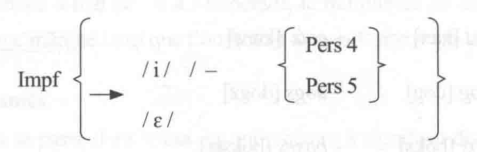
\includegraphics[width=.54\linewidth]{assets/ch09_imparfait_original.png}\end{center}

\minititle{2. L’exemple du verbe « aller » en français}
Le lexème « aller » reçoit en français :
\origpage{252}{238}
\begin{itemize}
\item le signifiant /i/ quand il précède le morphème du futur : « irai », « iras », etc.
\item le signifiant /v/ au présent avec les morphèmes de la 1ère, 2ème, 3ème et 6ème personne : « vais », « vas », « va », « vont » etc.
\item Le signifiant /al-/ au présent (quand il se combine directement avec les morphèmes de la 4ème personne et de la 5ème personne ( « allons », « allez ») et au subjonctif présent ( « allions », « alliez »)
\end{itemize}
Dans tous ces cas, c’est la présence de tel ou tel morphème grammatical qui entraîne la variation. Ainsi, on dira qu’un verbe conjugué se réalise sous la forme de plusieurs allomorphes : « all- », « i- », « v ».

\minititle{3. L’exemple allomorphie affixale : le préfixe privatif « / \bipa{ɛ̃} / » en français}
Toujours en français, le préfixe privatif / \bipa{ɛ̃} / ( « in- ») peut, en fonction du contexte, prendre des formes diverses mais de sens identique. Regardons le corpus ci-dessous :
\begin{center}\begin{tabular}{ll}
$\diamond$\quad inacceptable & $\diamond$\quad introuvable\\
$\diamond$\quad immoral & $\diamond$\quad immobile\\
$\diamond$\quad immangeable & $\diamond$\quad impossible\\
$\diamond$\quad imbuvable & $\diamond$\quad illogique\\
$\diamond$\quad irréel & $\diamond$\quad irremplaçable
\end{tabular}\end{center}
Dans ce corpus, chacune des unités partage le signifié privatif « qui n’est pas », mais sa manifestation au niveau de l’expression formelle présente des variations. Ce signifié possède trois allomorphes : « in- », « im- », et « ir- » ne correspondant qu’à un seul morphème. Ici encore, le locuteur ne choisit pas la variante, elle s’impose à lui.\ednote{原列 illogique 还显示 il-，所以按所列拼写变体应有4种而非3种。此外“语素异形态”是同一语素的形式变体，不是 signifié 自身具有多种形式；应改为 ce morphème possède…。标题 L’exemple allomorphie 缺 d’。}

\minititle{4. L’exemple du morphème de la pluralité en anglais}
Les grammaires anglaises signalent que le pluriel reçoit trois marques principales différentes, à savoir [s], [z], [iz], auxquelles on ajoute une marque moins importante : \bipa{[ən]}. Le morphème de la pluralité est associé à quatre signifiants différents, et possède trois allomorphes. Cela est illustré dans les exemples suivants :
\begin{itemize}
\item \bipa{[s]}\quad : \textit{cat} \bipa{[kæt]}\qquad $\sim$ \textit{cats} \bipa{[kæts]}
\item \bipa{[z]}\quad : \textit{dog} \bipa{[dog]}\qquad $\sim$ \textit{dogs} \bipa{[dogz]}
\item \bipa{[iz]} : \textit{box} \bipa{[boks]}\qquad $\sim$ \textit{boxes} \bipa{[boksiz]}
\item \bipa{[Ɔn]} : \textit{ox} \bipa{[ɑks]}\qquad $\sim$ \textit{oxen} \bipa{[oksən]}
\end{itemize}
\ednote{紧邻上下文均说4种，trois allomorphes 应为 quatre allomorphes。末条方括号内首字底本近似 \bipa{Ɔ}，与上文和 oxen 内部的 ə 不同，应为 [ən]。英语各词的元音还涉及口音及旧式转写，不能将不同口音的转写规范混用。}
En plus des quatre allomorphes vus plus haut, et pour être complet, notez qu’il existe aussi ce qu’on \origcont{253}{239}appelle des formes de remplacement, comme par exemple :
\begin{itemize}
\item /e $\leftarrow$ (ae)/\quad :\quad man $\rightarrow$ men\qquad woman $\rightarrow$ women
\item /i: $\leftarrow$ (u)/\quad :\quad foot $\rightarrow$ feet\qquad tooth $\rightarrow$ teeth
\item /aj $\leftarrow$ (aw)/\quad :\quad mouse $\rightarrow$ mice\qquad louse $\rightarrow$ lice
\end{itemize}
\ednote{woman / women 的重读元音通常为 \bipa{/ʊ/} 与 \bipa{/ɪ/}，不能归入 man / men 的 \bipa{/æ/} 与 /e/ 交替。第一行把两组词套用同一替换式有误。原来用 aj、aw 的转写保留，不作逐字现代化替换。}
On appelle « apophonie » ces formes de remplacement. Nous allons y revenir en détail un peu plus bas avec des exemples tirés d’une autre germanique, l’allemand.\ednote{d’une autre germanique 缺名词 langue，应为 d’une autre langue germanique。}

\subsection{Le morphème et ses difficultés de segmentation}
Une première complication de l’analyse morphématique vient de ce qu’un signifié peut être associé, non pas à aucun signifiant, mais à une absence de marque formelle.

\minititle{\textcircled{\scriptsize 1} Morphème à signifiant zéro}
Dans le cas mentionné plus haut, les manuels d’analyse morphologique parlent facilement de « morphème zéro », mais cela peut prêter à confusion. En effet, il ne s’agit pas de morphèmes qui n’ont pas de signifiant (car un morphème doit, par définition, avoir et un signifié et un signifiant), mais de morphèmes qui ont pour signifiant une absence de marque formelle. Il serait donc plus juste de les appeler « morphèmes à signifiant zéro », c’est-à-dire des morphèmes dont le « silence » signifie quelque chose. Prenons des exemples et comparons les énoncés suivants :
\begin{itemize}
\item Nous mangions \bipa{/mɑ̃ʒ-j-ɔ̃/}
\item Nous mangerons \bipa{/mɑ̃ʒ-r-ɔ̃/}
\item Nous mangeons \bipa{/mɑ̃ʒ-ø-ɔ̃/}
\item Mangeons ! \bipa{/mɑ̃ʒ-ø-ɔ̃/}
\end{itemize}
Les deux derniers énoncés (« nous mangeons » et « mangeons ») comportent chacun un morphème à signifiant zéro /ø/ qui indique le présent et s’oppose :
\begin{itemize}
\item Au morphème /j/ qui indique l’imparfait (« -ions »)
\item Au morphème /r/ qui indique le futur simple ( « -rons »)
\end{itemize}
De même, dans l’énoncé « mange ! » à l’impératif, le morphème /ø/ de la terminaison verbale s’oppose au morphème marqué /ons/ que l’on trouve dans la forme au pluriel « mangeons ! ».\ednote{原文用 ø 表示零实现，勿与国际音标的圆唇前元音 [ø] 混同，宜使用 $\varnothing$；/ons/ 又混入拼写，若用音标应为 \bipa{/ɔ̃/}。Nous 开头三行的斜线中仅转写动词而省略主语 /nu/，不能当作整个句子的完整音标。}

\minititle{\textcircled{\scriptsize 2} Morphèmes amalgamés}
À l’opposé de ce qui se passe dans le cas des morphèmes à signifiant discontinu (où pour rappel un seul signifié est associé à deux ou plusieurs éléments de signifiant), il peut arriver que deux signifiés différents soient associables à un seul et même segment formel. Prenons un exemple :
\begin{quote}\textbf{Ex :} il va au marché \bipa{/il va o maʁʃe/}\end{quote}

\origpage{254}{240}
Le morphème /o/ « au » est bien sûr formellement non segmentable car il s’agit d’un seul phonème. Or, il correspond à deux signes linguistiques distincts, comme le montre la commutation de « marché » avec « hôpital » et « maison » :
\begin{itemize}
\item Il va \textbf{au} marché \bipa{/il va o maʁʃe/}
\item Il va \textbf{à l’}hôpital \bipa{/il va a lɔpital/}
\item Il va \textbf{à la} maison \bipa{/il va a la mɛzɔ̃/}
\end{itemize}
La commutation a permis de faire apparaître « au » /o/ sous sa forme indépendante et non amalgamée. Le linguiste et anthropologue américain \textbf{Charles Hockett} (1916-2000) le traite comme un morphème qui appartient simultanément à deux (ou, théoriquement, plusieurs) morphèmes, et a simultanément la signification des deux.\ednote{按本节所举 au = à + le 的分析，共同的 /o/ 形式应称 morph（形素）或融合实现，而非“一个 morphème 同时属于两个 morphèmes”。此处需要区分实现形式与被实现的语法单位；例词保持原样。}

\minititle{\textcircled{\scriptsize 3} L’apophonie, forme de remplacement}
Revenons à présent sur l’apophonie. On parle d’apophonie lorsqu’un signifié peut avoir pour signifiant, non pas un segment formel considéré en lui-même, mais le remplacement d’un segment formel par un autre segment formel. On en a vu quelques exemples avec le pluriel anglais. En voici d’autres avec le prétérit (passé) allemand.

En allemand, on l’a vu plus haut, le verbe \textit{singen} signifie « chanter ». Au prétérit, « je chantais » se dit : \textit{Ich sang}.

C’est la présence d’une voyelle de remplacement (/a/) qui indique que « Ich sang » est un prétérit. Cette forme de prétérit se retrouve dans de très nombreux verbes irréguliers allemands, comme par exemple :
\begin{itemize}
\item \textit{binden} « lier » $\rightarrow$ \textit{band}
\item \textit{dringen} « pénétrer » $\rightarrow$ \textit{drang}
\item \textit{finden} « trouver » $\rightarrow$ \textit{fand}
\item \textit{trinken} « boire » $\rightarrow$ \textit{trank}
\item \textit{sterben} « mourir » $\rightarrow$ \textit{starb}
\item \textit{essen} « manger » $\rightarrow$ \textit{aß}
\item \textit{treffen} « rencontrer » $\rightarrow$ \textit{traf}
\end{itemize}
Pour être précis, ce n’est pas seulement la voyelle /a/ qui indique le passé, mais le \textit{remplacement} du /i/ du signifiant du lexème par la voyelle /a/. C’est pour cela que l’on parle alors de forme de remplacement. Dans notre exemple, elle est notée /a$\leftarrow$(i)/ et se lit : « la voyelle /a/ remplace /i/ ». Dans les trois derniers exemples ci-dessus, je vous invite à noter un autre cas de figure : /a$\leftarrow$(e)/.

Notez enfin que l’anglais étant une langue germanique, on retrouve évidemment un phénomène \origcont{255}{241}d’apophonie dans le prétérit des verbes irréguliers :
\begin{itemize}
\item take $\rightarrow$ took
\item find $\rightarrow$ found
\item fight $\rightarrow$ fought
\end{itemize}

\section{LA MORPHOLOGIE LEXICALE}
À partir de lemmes existants, commento « fabrique »-t-on de nouveaux lemmes ?\ednote{commento 应为 comment，为明显赘字。} Selon la nature des morphèmes constitutifs des unités complexes, les procédés de construction lexicale sont regroupés en deux grands ensembles : la dérivation, que nous connaissons déjà un peu, et la composition.

\subsection{La dérivation}
Dans son \textit{Lexique de la terminologie linguistique} (1951), le linguiste et latiniste \textbf{Jules Marouzeau (1878-1964)} définit ainsi la dérivation :
\begin{quote}\small\itshape
Procédé par lequel on forme un mot nouveau en prenant pour base une racine, un thème, ou un mot existant. La dérivation procède habituellement par addition de suffixe (nation, national) ou par substitution (vanter, vant-ard).
\end{quote}
André Martinet, quant à lui, définit la dérivation comme une opération qui consiste à construire une unité complexe à partir d’un morphème libre (ou « libérable ») et d’un morphème lié (affixe). Il définit les morphèmes (monèmes) « libérables » et « conjoints » ainsi :
\begin{quote}\small\itshape
Certains monèmes sont toujours conjoints. Tel est, par exemple, le « -té » de gaieté qui n’apparaît jamais que dans des complexes de ce type. D’autres peuvent être libres ou conjoints selon les cas : « gai » est libre dans « il est gai », mais conjoint dans « gaieté », « donn(e) » est libre dans « il donne », mais est conjoint dans « donneur ». On peut les désigner comme libérables : dans « tendrement », « tendre- » est libérable puisqu’il existe hors des complexes du type « tendrement »; « -ment » ne l’est pas, qui n’existe que dans de tels complexes.
\end{quote}
On peut dire qu’il existe trois types de dérivation : la dérivation affixale, la dérivation parasynthétique, et la dérivation impropre (appelée conversion).

\minititle{\textcircled{\scriptsize 1} La dérivation affixale}
Si, en français, la dérivation affixale se fait à travers l’ajout de préfixes et/ou de suffixes à un lexème, il existe dans d’autres langues différents types d’affixes : préfixes, suffixes, infixes, circonfixes, interfixes, transfixes et supra fixes.

\minititle{1. Les préfixes}
Les préfixes sont des affixes antéposés à la base verbale ou lexicale, comme « dé- » dans « défaire » \origcont{256}{242}et « re- » dans « refaire ». Nous le savons, les préfixes ne provoquent jamais de changement de catégorie grammaticale de la base.

\minititle{2. Les suffixes}
Les suffixes sont des affixes postposés à la base, comme « -iste » dans le « fleuriste » ou « -able » dans « envisageable ». Les suffixes peuvent entraîner un changement de catégorie grammaticale de la base.

\minititle{3. Les infixes en grec, tagalog et bontoc et indonésien}
Comme son nom l’indique, un infixe s’insère à l’intérieur du radical. Par exemple, en grec, l’énoncé {\BBSixGreek λαμβάνω} (« je prends ») comprend :
\begin{itemize}
\item Une racine verbale ({\BBSixGreek λαϐ-})
\item Un suffixe ({\BBSixGreek -άνω}) inchoatif, indiquant que l’action commence
\item Un infixe inchoatif (-{\BBSixGreek μ}-), inséré à l’intérieur de la base ({\BBSixGreek λαϐ}$\rightarrow${\BBSixGreek λαμϐ}).
\end{itemize}
En \textit{tagalog}, une des cent soixante dix langues parlées aux Philippines, on utilise l’infixe « -um- » pour créer des verbes à partir de noms ou d’adjectifs. Par exemple, le verbe \textit{kumain} (« manger ») a été obtenu en ajoutant l’infixe « -um- » dans la base nominale \textit{kain} ( « la nourriture »). De la même façon, l’emprunt anglais \textit{graduate} est devenu \textit{grumaduate}.

En langue \textit{bontoc} (un autre dialecte des Philippines), \textit{fikas} (« fort ») a donné \textit{fumikas} (« être fort »), \textit{kilad} (« rouge ») a donné kumilad (« être rouge »), etc.

L’indonésien, comme le tagalog et le bontoc, est une langue austronésienne. Il est donc aussi très riche en infixes. En voici quelques exemples :
\begin{itemize}
\item \textit{Gembung} ( « rempli d’air ») $\rightarrow$ \textit{gelembung} ( « bulle »).
\item \textit{Cerlang} ( « lumière ») $\rightarrow$ \textit{cemerlang} ( « brillant »)
\item \textit{Gigi} ( « dents ») $\rightarrow$, \textit{gerigi} ( « dentelé »).
\item \textit{Dulu} ( « vieux ») $\rightarrow$ \textit{dahulu} ( « autrefois »)
\item \textit{Kerja} ( « travail ») $\rightarrow$ \textit{kinerja} ( « performance »).
\end{itemize}
\ednote{同属南岛语系不足以推出某语言“中缀很丰富”；具体形式还须区分共时能产中缀、固化词形和借用构词。原书未给出这些印尼语例子的分析来源，这一因果推断尚不能确证。}

\minititle{4. Les circonfixes en allemand et indonésien}
Les circonfixes se placent autour d’un radical. En allemand, le participe passé est construit avec le circonfixe « ge-...-t ». Le verbe \textit{haben} (« avoir ») devient « gehabt » (« eu »), \textit{sagen} (« dire ») devient « gesagt », \textit{wollen} (« vouloir ») devient \textit{gewollt} (« voulu »), etc.\ednote{ge-…-t 只适用于一部分德语第二分词；强变化动词常以 -(e)n 结尾，有些动词没有 ge-，不能概括所有过去分词。此处举例本身可保留，应缩小概括范围。参见\ecite{50}。}

En indonésien, et dans bon nombre d’autres langues austronésiennes, il existe de très nombreux circonfixes, comme « \textbf{per-...-an} », qui marque la transformation nominale d’une base verbale. Par
\origcont{257}{243}exemple, le verbe \textit{janji} « promettre » donne \textit{perjanjian} (« promesse »). Le circonfixe « ke...an » marque la transformation d’un adjectif en nom :
\begin{itemize}
\item \textit{baik} (« bon ») $\rightarrow$ \textit{kebaikan} (« la bonté »)
\item \textit{cantik} (« beau, belle ») $\rightarrow$ \textit{kecantikan} (« la beauté »)
\item \textit{kaya} (« riche ») $\rightarrow$ \textit{kekayaan} (« la richesse »)
\end{itemize}

\minititle{5. Les interfixes en français et allemand}
Revenons à présent un instant au français avec l’interfixe, un type d’affixe dépourvu de valeur sémantique qui s’intercale (d’où son nom) entre deux morphèmes, comme dans « fermeture », « obscurantisme », « puisatier », « sauvetage », etc. On retrouve souvent les interfixes en français pour relier les racines grecques et latines, comme dans « mythomane » ou « chimiothérapie », etc. C’est ce qu’on appelle la composition savante, et je vais y revenir en détail un peu plus bas.

En allemand, l’interfixe intervient dans la formation des mots composés :
\begin{itemize}
\item \textit{Arbeitszimmer} (« bureau ») est composé de \textit{Arbeit} (« travail ») et de \textit{Zimmer} (« une pièce de la maison »), reliés par le transfixe « s ».
\item \textit{Arbeitslos} (« chômeur »), est composé de \textit{Arbeit}, du transfixe « s », et du suffixe « los » (« dépourvu de »).
\end{itemize}
\ednote{两例中的“transfixe”与本小节自己的术语不一致，应作 interfixe（连接成分）。德语 arbeitslos 是形容词“失业的”，并非名词 chômeur 的直接对应；作名词时须用相应的名词化形式。}
Notez néanmoins que ce n’est pas une règle absolue. Le synthème « chambre à coucher » (\textit{Schlafzimmer}) est composé de \textit{schlafen} (« dormir ») et de \textit{Zimmer}, sans interfixe.

\minititle{6. Les suprafixes en langue ngbaka}
Dernier cas de figure, le suprafixe est un type d’affixe qui ajoute une unité suprasegmentale (autrement dit, un ton ou un accent tonique) à une base neutre pour donner un sens dérivé ou fléchi. Le terme de suprafixe a été suggéré par le linguiste et traducteur américain \textbf{Eugene Nida} (1914-2011) mais il est peu employé, et certains linguistes préfèrent le terme de « superfixe ». Nous avons déjà vu que le plupart des langues africaines sont tonales, et bon nombre de langues africaines marquent une différence de temps ou d’aspect à l’aide d’un suprafixe. Le ngbaka, langue d’Afrique centrale, possède trois suprafixes marqués par trois signes diacritiques différents : la voix aiguë est marquée par un accent aigu, la voix moyenne est marquée par un macron (ō), la voix basse est marquée par un accent grave. Comme en chinois, un changement de suprafixe en ngbaka entraîne un changement de sens :
\begin{itemize}
\item \bipa{sɔ́} ton haut : « animal »
\item \bipa{sɔ̄} ton moyen : « chasser »
\item \bipa{sɔ̀} ton bas : « queue »
\end{itemize}
\ednote{“le plupart”应作 la plupart。这里三例只显示词汇声调对立，尚不能仅凭例子证明它们是同一词基加上语法性超音段词缀的派生关系；原书把声调与 suprafixe 直接等同，需加此分析限度。}

\origpage{258}{244}
\minititle{\textcircled{\scriptsize 2} La dérivation parasynthétique}
On parle de dérivation parasynthétique à propos de lemmes qui comportent \textit{simultanément} un préfixe et un suffixe. J’attire votre attention sur l’adverbe \textit{simultanément} : dans le cas de la dérivation parasynthétique, aucun des affixes ne peut s’ajouter seul à la base. Prenons l’exemple du verbe « aguerrir », obtenu par dérivation parasynthétique. Le verbe « *guerrir » n’existe pas, « *aguerre » non plus. Voici des exemples de mots construits par dérivation parasynthétique. Dans le tableau ci-dessous, notez la présence d’interfixes et de formes de remplacement étudiés plus haut :
\begingroup\small
\begin{longtable}{p{.12\linewidth}p{.22\linewidth}p{.16\linewidth}p{.34\linewidth}}
\toprule\textbf{Préfixe}&\textbf{Base}&\textbf{Suffixe}&\textbf{Dérivé parasynthétique}\\\midrule\endfirsthead
\toprule\textbf{Préfixe}&\textbf{Base}&\textbf{Suffixe}&\textbf{Dérivé parasynthétique}\\\midrule\endhead
en&col&ure&encolure\\
é&clair&er, cir&éclairer, éclaircir\\
a&mer (+r)&ir&amerrir\\
en&courage&er&encourager\\
dé&courage&er&décourager\\
a&peur&er&apeurer\\
a&lune&ir, issage&alunir, alunissage\\
en&flamme&er&enflammer\\
dé&rat&iser&dératiser\\
en&four (+n)&er&enfourner\\
em&bourgeois&er&embourgeoiser\\
a&doux (+c)&ir&adoucir\\
en&diable&er&endiabler\\
dés&herbe&er&désherber\\
en&dimanche&er&endimancher\\
rem&bourse&er&rembourser\\
é&rein (+t)&er&éreinter\\
ra&court (+c)&ir&raccourcir\\
é&borgne&er&éborgner\\
en&riche&ir&enrichir\\\bottomrule
\end{longtable}
\endgroup
\ednote{表中项目不全满足上文“两个词缀必须同时加入”的标准。例如 alunissage 可以由同表已有的 alunir 再派生，并不能作为不存在中间形式的例证。正文与表格均照录，不将整表都视为已确证的同步加缀分析。}

\minititle{\textcircled{\scriptsize 3} La dérivation impropre (conversion)}
La dérivation « impropre », appelée aussi conversion, est un procédé de formation de mot au moyen duquel le mot change de catégorie grammaticale sans aucune modification formelle : elle est donc aussi appelée « dérivation zéro ». Considérée comme un des procédés les plus productifs en français moderne, il en existe trois formes : la substantivation, l’adjectivation, l’adverbialisation.

\origpage{259}{245}
\minititle{1. La substantivation}
La substantivation (ou nominalisation) consiste à transformer en substantif un mot qui n’appartient pas originellement à cette catégorie, notamment :
\begin{itemize}
\item un adjectif : le beau, le vrai, un bleu, le pauvre, un Français, un noir, etc.
\item un participe passé : un employé, un handicapé, un névrosé, un abruti, un poilu, un vendu, un élu, etc.
\item un verbe à l’infinitif : le manger, le boire, le dîner, le coucher, le savoir, le devoir, etc. A la différence du latin et du grec, seuls quelques verbes français peuvent être transformés en noms. Ainsi, « le vivre ensemble » est correct, alors « *le mourir dignement » ne l’est pas.
\end{itemize}
On peut aussi former des noms à partir d’autres noms. Vous allez le voir ci-dessous, c’est donc un procédé très économique.

\minititle{1) La métonymie}
En stylistique, la métonymie est un procédé qui consiste à nommer quelque chose à l’aide d’un terme qui en désigne un autre, mais qui a cependant avec le premier terme une relation logique. Avec la métonymie, on peut créer des noms communs :
\begin{itemize}
\item En désignant un produit par le nom de son lieu d’origine (toponyme) : un champagne (un vin de Champagne), un bourgogne (un vin de Bourgogne), un havane (un cigare cubain), un brie (un fromage de la région de Brie), un hamburger (de la ville de Hambourg), etc.
\item En désignant l’objet par la matière dont il est fait : un bronze de Rodin (eun sculpture en bronze),\ednote{“eun sculpture”应作 une sculpture。} une huile de Matisse (une peinture à l’huile), un jean (un pantalon en toile de jean), un feutre (un chapeau en feutre), un vison (un manteau en fourrure de vison), un fusain (dessin fait au fusain), une aquarelle, une encre de Chine, un plâtre, un verre, etc
\item En désignant le contenu par le contenant : boire un verre, prendre un pot, manger un plat, etc.
\item En désignant l’activité par le lieu où elle s’exerce : un théâtre, un café, un cinéma, un opéra, une cuisine, etc.
\item En désignant une institution par le lieu où elle se trouve : Bercy (le ministère français des finances), le quai d’Orsay (le ministère français des affaires étrangères), Matignon (la résidence du Premier Ministre), la Place Beauvau (le ministère de l’intérieur), la rue d’Ulm (École Normale Supérieure), etc.
\end{itemize}

\minititle{2) L’antonomase}
La substantivation permet aussi de transformer un nom propre (appelé aussi anthroponyme) en nom commun : c’est ce qu’on appelle une antonomase.\ednote{anthroponyme 专指人名，不是所有 nom propre（专名）的同义词；如本页已经出现的 toponyme 指地名。此处只在专名是人名时才成立。} Ces anthroponymes peuvent être tirés \origcont{260}{246}de :
\begin{itemize}
\item la mythologie : un narcisse, un pygmalion, un apollon, un sosie, un mentor, un argus, une chimère, un dédale, une harpie, un pactole, un amphitryon, une mégère, une panacée, etc.
\item la littérature : un dom juan, un harpagon, un rastignac, une dulcinée, un gavroche, un gargantua, etc.
\end{itemize}
Mais il peut aussi s’agir d’anthroponymes de personnes réelles :
\begin{itemize}
\item des artistes : lire un Balzac, acheter un Picasso, porter un Chanel, etc.
\item des personnages historiques : un mécène, une égérie, une messaline, un crésus, etc.
\item des savants qui ont laissé leur nom à des unités de mesure : un watt (James Watt) un ampère (André-Marie Ampère), un pascal (Blaise Pascal), un hertz (Heinrich Herz), un newton (Benjamin Newton), un becquerel (Henri Becquerel), etc...\ednote{两个人名有误：Heinrich Herz 应作 Heinrich Hertz；力的单位 newton 得名于 Isaac Newton，不是“Benjamin Newton”。参见\ecite{51}。}
\item des inventeurs : une poubelle (invention d’Eugène Poubelle, préfet de la Seine), un barème (François-Bertrand Barrême), le braille (Louis Braille), un diesel (Rudolf Diesel), une mansarde (François Mansart), une montgolfière (les frères Montgolfier), une rustine (Louis Rustin), la nicotine (Jean Nicot), etc.
\end{itemize}
Notez que dès que l’antonomase du nom propre se lexicalise, le nom propre devient un véritable nom commun autonome et s’écrit donc sans majuscule.

Ex : Ce jeune banquier est un mozart de la finance !

\minititle{2. L’adjectivation}
Comme son nom l’indique, l’adjectivation consiste à transformer en adjectif un terme qui n’appartient pas originellement à cette catégorie. Elle concerne quelques rares adverbes (l’étage au dessus, la voiture devant, c’est assez, etc.), mais principalement des noms, et les adjectifs tirés d’un substantif sont d’un emploi très large. On peut trouver des substantifs désignant la couleur (rose saumon, rouge bonbon, bleu ciel, vert pomme, etc.), mais pas seulement : un air canaille, une affluence monstre, un effet surprise, un discours fleuve, un enfant roi, une femme enfant, un bébé éprouvette, un tailleur couture, un regard assassin, un chapeau melon, une assurance vie, un portrait robot, etc. Vous le voyez, la liste est potentiellement très longue.

\minititle{3. L’adverbialisation}
En français, on peut créer de nombreux mots en employant des adjectifs comme des adverbes : rire jaune, voir rouge, parler fort, coûter cher, sentir bon, travailler dur, frapper sec, etc.\origfoot{4}{Dans le chapitre suivant, qui sera en grande partie consacré à la syntaxe fonctionnelle de \textbf{Lucien Tesnière}, nous reviendrons sur ces exemples de conversion : gardez-les bien à l’esprit.}

\origpage{261}{247}
Après la dérivation, passons à présent au second procédé de construction lexicale : la composition.

\subsection{La composition}
La composition est un procédé de construction lexicale qui permet de combiner deux lemmes (les composants) pour en former un nouveau (le composé). On distingue la composition ordinaire et la composition savante.

\minititle{\textcircled{\scriptsize 1} La composition ordinaire}
La composition la plus courante consiste à associer deux mots qui ont une existence autonome par ailleurs. Ils peuvent être soudés l’un à l’autre ( « porte » + « feuille » $\rightarrow$ « portefeuille »), reliés par une préposition (« machine à laver », « fruit de mer ») ou par un trait d’union (« arc-en-ciel », « tire-bouchon », « porte-avion »). Ce qu’il faut rappeler, c’est que sur le plan syntaxique un mot composé fonctionne comme un morphème unique (synthème). Sur le plan sémantique, il forme une unité de sens nouvelle qui dépasse celle des éléments pris isolément. N’appartenant qu’à seul un paradigme,\ednote{“qu’à seul un paradigme”应作 qu’à un seul paradigme。} lors d’une commutation, c’est donc tout le synthème qui commute, comme suit :

\noindent Ex :\par\smallskip
\noindent\begin{tabularx}{\linewidth}{@{}Xl@{}}
Je vais au marché acheter des&\underline{fruits de mer}\\
Je vais au marché acheter des&\underline{oignons}\\
Je vais au marché acheter des&\underline{chaussettes}\\
\end{tabularx}

La seule commutation de l’un ou l’autre des composants du synthème donnerait en effet des résultats, disons-le, assez inattendus :

\noindent Ex :\par\smallskip
\noindent\begin{tabularx}{\linewidth}{@{}Xll@{}}
Je vais au marché acheter des&\underline{fruits}&de mer\\
? Je vais au marché acheter des&\underline{tomates}&de mer\\
? Je vais au marché acheter des&\underline{fraises}&de mer\\
\end{tabularx}

\noindent Ex :\par\smallskip
\noindent\begin{tabularx}{\linewidth}{@{}Xl@{}}
Je vais au marché acheter des fruits de&\underline{mer}\\
? Je vais au marché acheter des fruits de&\underline{lac}\\
? Je vais au marché acheter des fruits de&\underline{rivière}\\
\end{tabularx}

\minititle{\textcircled{\scriptsize 2} La composition savante}
Lorsque la composition se fait à partir d’emprunts au latin et au grec, on parle de composition « savante ». En français, un nombre considérable de termes médicaux, techniques, scientifiques, linguistiques, philosophiques ont ainsi été formés. Appelée aussi « interfixation », la composition \origcont{262}{248}savante consiste à juxtaposer deux (ou plus) radicaux d’origine latine ou grecque (appelés étymons), et à ajouter éventuellement un suffixe pour préciser la catégorie ou le genre du mot ainsi composé.

Par exemple, c’est l’ajout d’un suffixe qui permet de distinguer la « biologie » (la spécialité) du « biologiste » (le spécialiste) et la « linguistique » du « linguiste ». A la différence de la composition ordinaire, les éléments d’origine latine ou grecque sont toujours juxtaposés et collés sans trait d’union. Les éléments servant à la composition peuvent être :
\begin{itemize}
\item tous les deux latins : apiculture, multicolore, homicide, ignifuge, calorifère, carnivore. Notez l’utilisation de l’interfixe « i », qui sert de lien entre les deux éléments d’origine latine.
\item tous les deux grecs : anthropologie, thalassothérapie, cryptomanie, démocratie, hydrogène, polymorphe, topographie, pyromane, gynécologue. Le lien entre deux deux lexèmes grecs est l’interfixe « o ».\ednote{“deux deux”叠印，应删去一个 deux。}
\item un latin et un grec :
\begin{itemize}
\item « télévision » est composé du grec \textit{teleo} (« loin ») et du verbe latin \textit{videre} (« voir »)\ednote{表示“远”的希腊语成分应为 {\BBSixGreek τῆλε}（tēle / têle），此处“teleo”有误。拉丁部分经由 vision 构成，不宜把现代词直接等同于两个未经中介的古语词的拼接。}
\item « automobile » vient du grec \textit{auto} (« soi-même ») et du latin \textit{mobilis} (« mobile »)
\item « génocide » vient du grec « genos » (race) et du latin \textit{caedere} (« tuer »)
\end{itemize}
\end{itemize}

\minititle{1. La place des étymons}
Certains de ces lexèmes peuvent apparaître librement en tête ou en queue de mot. Par exemple :
\begin{itemize}
\item cinéphile / philosophe
\item téléphone / phonologie
\item phonographe / graphologie
\item grammaire / calligramme
\item anthropologie / philanthrope
\end{itemize}
D’autres ne peuvent être utilisés qu’en début ou en fin de mot. Le lexème grec \textit{mane}, par exemple, ne peut se placer qu’à la fin du mot composé :
\begin{itemize}
\item érotomane
\item mélomane
\item mythomane
\item mégalomane
\item mythomane
\end{itemize}
\origpage{263}{249}
\begin{itemize}
\item nymphomane
\item pyromane
\end{itemize}
Quant à \textit{anti-}, \textit{archi-}, \textit{para-}, \textit{méta-}, ils ne peuvent apparaître qu’en début de mot. Dans les chapitres précédents, nous avons rencontré, souvenez-vous, les exemples suivants :
\begin{itemize}
\item \textit{anti}logie
\item \textit{archi}phonème
\item \textit{para}logisme, \textit{para}taxe
\item \textit{méta}langage, \textit{méta}physique
\end{itemize}
Leur place en début ou fin de mot pourrait donner l’impression qu’ils entrent dans la construction de mots dérivés, mais il ne s’agit pas de dérivation : ce ne sont pas des affixes, mais des lexèmes.

\minititle{2. L’allomorphie latine : les doublets}
Un doublet lexical (appelé aussi « doublon ») est une paire de mots qui diffèrent par la forme et par le sens, mais qui ont la même origine étymologique. Cette différence de forme et de sens est due au fait qu’ils sont entrés dans la langue par des voies différentes. En voici quelques exemples :
\begin{itemize}
\item le latin \textit{regalis} a donné « royal » par une évolution phonétique très lente, mais aussi « régalien » par emprunt direct au latin classique.
\item les deux adjectifs « fragile » et « frêle » illustrent également ce phénomène. Le premier, proche de l’étymon latin \textit{fragilis}, est issu de la dérivation savante, le second relève de la dérivation populaire.
\item « nager » et « naviguer » sont deux formes allomorphiques du même étymon latin \textit{navigare}.
\item les lemmes « hôtel » et « hôpital » viennent tous deux du latin \textit{hospitalis}.
\end{itemize}
\ednote{这里描述的是不同词位的历时词源双式，不是本章此前所定义的“同一语素的不同实现”意义上的共时异形态。“allomorphie”在此被扩大使用，应与词源关系区别；下文“voie populaire / voie savante”比“dérivation populaire / savante”更准确地概括本段自己的说明。}
Les mots plus éloignés du latin ( « royal », « hôtel » et « frêle ») ont subi des transformations phonétiques, alors que les autres, plus proches du latin ( « régalien », « hôpital » et « fragile ») ont été puisés directement dans le bas-latin et adaptés en langue romane. Les doublets proviennent donc d’un même mot latin soit par évolution phonétique (voie populaire), soit par emprunt direct (voie savante). Leurs significations peuvent être proches ou éloignées : comment en effet imaginer que « penser » et « peser » viennent du même etymon \textit{pendere} ? En tout cas, cela explique l’expression « peser le pour et le contre ». Voici d’autres exemples, non exhaustifs bien sûr :

\origpage{264}{250}
\begin{longtable}{p{.27\linewidth}p{.29\linewidth}p{.29\linewidth}}
\toprule\textbf{Mots latin}&\textbf{Évolution phonétique}&\textbf{Emprunt direct}\\\midrule\endfirsthead
\toprule\textbf{Mots latin}&\textbf{Évolution phonétique}&\textbf{Emprunt direct}\\\midrule\endhead
\textit{regalis}&royal&régalien\\
\textit{acrem}&aigre&âcre\\
\textit{rigidus}&raide&rigide\\
\textit{fragilis}&frêle&fragile\\
\textit{legalis}&loyal&légal\\\midrule
\textit{pendere}&peser&penser\\
\textit{integer}&entier&intègre\\
\textit{fabrica}&forge&fabrique\\
\textit{masticare}&mâcher&mastiquer\\
\textit{auscultare}&écouter&ausculter\\\midrule
\textit{potio}&poison&potion\\
\textit{maturus}&mûr&mature\\
\textit{captivus}&chétif&captif\\
\textit{navigare}&nager&naviguer\\
\textit{articulus}&orteil&article\\
\textit{captivum}&chétif&captif\\\bottomrule
\end{longtable}
\ednote{表头“Mots latin”应为 Mots latins。“captivus / captivum”两行的法语结果相同，底本确实重复列出，故不合并。词源表中的拉丁形式与借入年代还需逐项核对，不据此表直接推出每对词的具体传播途径。}

\minititle{3. Le supplétisme}
En morphologie, on parle de supplétion quand l’ensemble des formes que prend un même lemme (son paradigme) fait intervenir plusieurs radicaux (ou lexèmes) d’origine différente mais de sens voisin, au lieu d’être basé sur les modifications (flexions) d’un unique radical. Il s’agit d’une irrégularité, d’une exception à la règle qui rend imprévisible la flexion du mot considéré.

\minititle{1) L’exemple du verbe « aller »}
Nous avons déjà, sans le savoir, évoqué le supplétisme un peu plus haut avec les allomorphes du verbe « aller ». La première personne du singulier du verbe « aller » est « je vais », et non pas, comme on pourrait intuitivement s’y attendre, « *j’alle ». De même, au futur, la première personne du singulier du verbe « aller » est « j’irai », et non « *j’allerai ». Cela, nous le savons déjà. Mais à présent, je peux vous expliquer pourquoi :
\begin{itemize}
\item les formes en « all- » sont bâties sur l’étymon latin \textit{alare}
\item les formes en « va » proviennent du verbe latin \textit{vadere}
\item les formes en « ir- »viennent du verbe latin \textit{ire}
\end{itemize}
\ednote{“alare”在此作为已确证拉丁词源给出，缺乏依据；aller 的词源涉及拟构与音变分析，不能把未注明拟构性质的 alare 当作无争议实证。词源仍待核。}
Dans le cas du supplétisme, les bases sont trop distantes pour parler d’allomorphie, car la flexion ne consiste donc plus seulement en une \textit{modification} du lexème, comme dans le cas d’allomorphie, mais de son \textit{remplacement} par un autre : les radicaux, dits « supplétifs » remplacent le radical usuel de même sens, mais indisponible.

\minititle{2) L’exemple de l’adjectif « ludique »}
Dans le processus de dérivation, il arrive que des voyelles de la racine lexicale subissent un changement. Ce processus, appelé alternance vocalique, est parfois prévisible :

\origpage{265}{251}
« cœur $\rightarrow$ cordial », « fleur $\rightarrow$ floral », « mœurs $\rightarrow$ moral », « liqueur $\rightarrow$ liquoreux », « chœur $\rightarrow$ chorale », « heure $\rightarrow$ horaire », « professeur$\rightarrow$professorat »

Dans le cas du substantif « jeu », on ne peut pas prévoir cette altération formelle. Dans l’adjectif « ludique » («relatif au jeu»), on retrouve manifestement le suffixe adjectival « -ique », mais il n’existe pas de substantif « *lude », auquel s’ajouterait ce suffixe.

En fait, pour des raisons phonétiques, il est difficile de créer un adjectif basé sur « jeu » (en latin, \textit{jocus}). On a donc créé l’adjectif « ludique », phonologiquement non motivé, et basé sur un autre étymon latin : « \textit{ludus} » ( le jeu). On dit alors que « ludique » entretient un rapport supplétif avec « jeu ». Ce sont, en quelque sorte, des « parents par alliance ».

\minititle{3) Autres exemples}
Sans connaissance de l’étymologie, difficile de faire la distinction entre l’allomorphie et le supplétisme, mais globalement l’opposition entre l’allomorphie et le supplétisme peut être définie comme une variation régulière (allomorphie) et singulière (supplétisme) de la base. Voici d’autres exemples de radicaux supplétifs :
\begin{itemize}
\item Le verbe « incarcérer » est construit sur la racine latine \textit{carcer} parce que « emprisonner » a un sens métaphorique. L’adjectif « carcéral » est lui aussi construit sur la même racine latine. Le substantif « prison » vient d’une autre racine latine : \textit{prehensio} ( « prendre »).
\item Le substantif « maison » vient de latin \textit{mansio}. L’adjectif « domestique » est basé un autre étymon latin, \textit{domus}, de même sens.
\item Le fait d’être aveugle est appelé « cécité », parce qu’« aveuglement » existe déjà, mais avec un sens figuré. « Cécité » est basé sur l’étymon latin \textit{caecitas}. « Aveugle » est basé sur un autre étymon latin, de même sens : \textit{ab oculis}.
\end{itemize}
\ednote{本段“basé un autre”缺少 sur，应作 basé sur un autre。incarcérer 与 emprisonner 均可用于实指监禁，不能以“emprisonner 具有比喻义”作为前者产生的充分原因。此处不同来源的相关词与前页同一屈折范式中的补充关系，也应在分析层次上分开。}
Quittons le latin et de faire un saut dans le temps pour revenir à l’époque moderne.\ednote{“et de faire”应作 et faisons，与 Quittons 构成并列祈使句。} Après la dérivation et la composition, nous allons nous intéresser à un autre moyen très efficace de création lexicale : les sigles et les acronymes.

\subsection{Siglaison et acronymisation}
Au quotidien, dans nos productions langagières, nous tendons tout naturellement à limiter notre effort articulatoire : c’est ce qu’on appelle la loi du moindre effort articulatoire. Prononcer « Institut national de la statistique et des études économiques ou « INSEE », ce n’est pas le même effort articulatoire. Heureusement, pour limiter notre effort et économiser notre salive, le français dispose de sigles et acronymes très nombreux.

\minititle{\textcircled{\scriptsize 1} Le sigle}
Le sigle est un terme composé de la succession des initiales des termes qui le composent. Ces initiales doivent prononcées une à une, et non pas comme un mot.\ednote{“doivent prononcées”应为 doivent être prononcées。前段 Institut…économiques 后遗漏右引号。} En voici quelques exemples :

\origpage{266}{252}
\begin{itemize}
\item Un V.T.T. : un vélo tout-terrain
\item Un S.D.F. : un sans domicile fixe
\item Un C.D.I. : un contrat à durée indéterminée
\item L’I.S.F. : l’impôt de solidarité sur la fortune
\item Une I.V.G : une interruption volontaire de grossesse
\item Le F.M.I. : le Fonds Monétaire International
\item La P.M.A : la procréation médicalement assistée
\end{itemize}
La siglaison peut faire l’objet d’une dérivation :
\begin{itemize}
\item Un RMIste est une personne percevant le R.M.I. (Revenu Minimum d’Insertion)
\item Un VTTiste est un amateur de V. T. T.
\item Un CGTiste est un membre de la CGT (Confédération Général du Travail)\ednote{名称中的 Général 应作 Générale，与阴性名词 Confédération 配合。这些机构、福利和制度名称在本章作为词汇构造实例保留，不代表本重排版断言其仍全部维持出版时的制度状态。}
\end{itemize}

\minititle{\textcircled{\scriptsize 2} L’acronyme}
Un acronyme est un mot formé des initiales (OTAN) ou des éléments initiaux (le Bénélux) de plusieurs mots. A la différence du sigle, il se prononce comme un mot normal et non pas lettre par lettre. Un acronyme peut s’écrire, selon le cas :
\begin{itemize}
\item Comme un sigle, entièrement en lettres capitales, et sans points de séparation, s’il est constitué d’initiales. Par exemple : la COFACE (Compagnie française d’assurance pour le commerce extérieur), le MEDEF (Mouvement des entreprises de France), l’ENA (École Nationale d’Administration), la FIFA (La Fédération internationale de football association), les D.O.M.-T.O.M. (départements d’outre-mer et territoires d’outre-mer), l’ONU (Organisation des Nations Unies)
\item Comme un nom propre, avec une majuscule. Par exemple : le Benelux (\textit{Belgium, Netherland, Luxembourg}), le Mercosur (de l’espagnol \textit{Mercado Común del Sur}), le Gatt (\textit{General Agreement on Tariffs and Trade}), etc.\ednote{英语国家名应为 Netherlands，而不是 Netherland；这里保留底本对 Benelux 构成的说明形式。}
\item Comme un nom commun, en minuscules, s’il est lexicalisé. Par exemple : un laser (\textit{light amplification by stimulated emission of radiation}), un radar (\textit{radio detection and ranging}), le sida (syndrome d’immunodéficience acquise,), un ovni (objet volant non identifié), le pacs (pacte civil de solidarité), etc.
\end{itemize}
Comme le sigle, l’acronyme peut lui aussi être lexicalement « dérivé » et servir de racine à de nouveaux termes lexicaux (noms, adjectifs et verbes). Ainsi :

\origpage{267}{253}
\begin{itemize}
\item La science qui étudie les ovnis est appelée «ufologie»,\origfoot{5}{\textit{ufo} en anglais, est l’acronyme d’\textit{unidentified flying object}.} et le spécialiste de cette science est un « ufologue ». C’est un bel exemple de supplétisme : « *ovnilogue » n’étant pas possible, on lui a substitué un radical anglais de sens identique.
\item Une personne qui perçoit le SMIC est un smicard.
\item Un ancien étudiant de l’ENA est un énarque.
\item Un programme de l’ONU est un programme onusien.
\item Un couple qui a signé un PACS pour « se pacser » est un couple « pacsé ».
\end{itemize}

\subsection{Troncation et métaplasmes par soustraction}
La loi du moindre effort articulatoire évoquée plus haut est une tendance générale constatée dans l’évolution des langues selon laquelle certains traits phonétiques, dont le coût en termes d’effort articulatoire est important, tendent à s’user ou à disparaître. Chercher à raccourcir les mots pour limiter l’effort articulatoire est une tendance générale et naturelle. Parmi les moyens dont nous disposons, il y a la troncation (du latin \textit{truncare}, trancher, amputer) procédé utilisé pour réduire un lemme, pour créer des diminutifs hypocoristiques (autrement dit, des termes tendres et affectueux) ou des abréviations.

Les éléments tronqués peuvent être :
\begin{itemize}
\item laissés de la sorte : un prof, un bus, la télé
\item suffixés : le directeur $\rightarrow$ le dirlo
\item dupliqués : un communiste $\rightarrow$ un coco
\end{itemize}
Ces altérations, autorisées par l’usage, sont appelées « métaplasmes ». Les différentes formes de troncation que je vais vous présenter ci-dessous sont des métaplasmes dite « par soustraction ».\ednote{“des métaplasmes dite”应为 des métaplasmes dits。}

\minititle{\textcircled{\scriptsize 1} La troncation par apocope}
En phonétique, une apocope (du grec \textit{apokoptein}, « retrancher ») est l’amuïssement d’un ou plusieurs phonèmes \textit{en fin d’un mot}. Par exemple :
\begin{itemize}
\item auto, pour \textit{automobile}
\item télé, pour \textit{télévision}
\item amphi, pour amphithéâtre
\end{itemize}
C’est la forme la plus courante de troncation.

\minititle{\textcircled{\scriptsize 2} La troncation par aphérèse}
L’aphérèse (du grec \textit{aphaíresis}, « ablation ») est un métaplasme impliquant l’amuïssement \origcont{268}{254}d’un ou plusieurs phonèmes \textit{en début de mot}. Peu fréquente, elle est utilisée dans les diminutifs hypocoristiques :
\begin{itemize}
\item Bastien (pour \textit{Sébastien})
\item Colas (pour \textit{Nicolas})
\item Sandre (pour \textit{Alexandre})
\item Toine (pour \textit{Antoine})
\item Tony (pour \textit{Antony})
\end{itemize}
L’aphérèse est aussi utilisée dans quelques termes devenus courants :
\begin{itemize}
\item un bus (pour \textit{autobus})
\item un car (pour \textit{autocar})
\item un chandail (pour \textit{marchand d’ail})
\item le \textit{net} (pour \textit{internet})
\item un ricain (pour \textit{Américains}).
\end{itemize}
À l’oral, des aphérèses peuvent se produire dans le registre familier, comme dans « blème » (problème). La langue française ne connaît que peu d’amuïssements à l’initiale. Retenez que c’est l’apocope qui domine dans l’évolution du français.

\minititle{\textcircled{\scriptsize 3} La troncation par syncope}
La syncope (du grec ancien \textit{synkopè}, « retranchement») est un métaplasme consistant en l’amuïssement d’un phonème (ou plus) \textit{à l’intérieur} d’un mot :
\begin{itemize}
\item « M’sieur », pour « monsieur »
\item « M’dame », pour « madame »
\item « Mam’selle », pour « mademoiselle »
\item « P’tit » pour « petit »
\end{itemize}
Notez que « Monsieur » est lui-même le résultat d’une syncope à partir de « monseigneur ».

\minititle{\textcircled{\scriptsize 4} La déglutination}
La déglutination est un cas un peu particulier de de métaplasme : il s’agit d’une aphérèse reposant sur une mauvaise segmentation (appelée mécoupure) d’un mot, compris \textit{à tort} comme s’il était précédé d’un article, alors que ce n’est pas le cas.\ednote{“de de métaplasme”叠印，应删去一个 de。}

Par exemple, en anglais, « tablier » se dit \textit{apron}. Ce mot anglais vient du français « napperon »,
\origcont{269}{255}emprunté puis mal coupé par la langue anglaise, comme suit :
\begin{itemize}
\item Étape 1 : emprunt direct du français en anglais$\rightarrow$ \textit{a napperon}
\item Étape 2 : déglutination (mauvaise coupe) $\rightarrow$ \textbf{\textit{an apron}}
\end{itemize}
Je vous donne deux autres exemples de déglutination :
\begin{itemize}
\item La fête religieuse française de l’« Ascension » est elle aussi le résultat d’une mauvaise coupe de la fête de « la Cencion ».\ednote{此例的方向疑被倒置：若由 l’Ascension 误切为 la Cension / la Cencion，才符合本段“去掉误认作冠词的词首成分”的定义；正文所述从 la Cencion 到 l’Ascension 并不能示范该过程。原书未给例证出处，此处仅作拟校。}
\item Le nom de la province française de la Guyenne vient du latin \textit{Aquitania} qui a d’abord donné « Aguienne » en ancien français, puis « l’Aguienne », et enfin « la Guyenne » au XIIIe siècle, le a- initial ayant été pris (par erreur) pour la voyelle finale de l’article « la ».
\end{itemize}

\subsection{Les métaplasmes par addition}
Les métaplasmes ci-dessus sont issus des travaux interdisciplinaires du \textbf{Groupe μ}, le Centre d’Études poétiques de l’Université de Liège. Les travaux que ce groupe poursuit depuis 1967 concernent la sémiotique et la poétique, mais aussi la rhétorique. Les métaplasmes par addition que l’on va voir à présent sont eux aussi issus des travaux du groupe μ, qui, vous allez le remarquer, semble avoir un goût prononcé pour la composition savante. Ne vous inquiétez-pas : le jargon est particulièrement hermétique, mais les idées sont simples.

\minititle{\textcircled{\scriptsize 1} La prosthèse}
La prosthèse consiste à ajouter un ou plusieurs phonèmes en début de mot. Par exemple, le mot français « étable » vient latin \textit{stabula}, « échelle » de \textit{scala}, « école » de \textit{scola}. La prosthèse se manifeste ici dans l’ajout du phonème /e/ en remplacement du phonème /s/ disparu au fil de l’évolution phonétique en français.\ednote{“vient latin”缺少 du。prosthèse 按本段自己的定义是词首增音，不能直接等同于“以 /e/ 替换 /s/”；词首增音与其后 /s/ 的消失是须区别的变化阶段。}

Notez qu’en anglais, pour les trois exemples ci-dessus (et bien d’autres, bien sûr), l’évolution phonétique est restée plus proche du latin que le français : dans \textit{stables}, \textit{school}, \textit{scale}, il n’y a pas de prothèse.

\minititle{\textcircled{\scriptsize 2} La paragoge}
Figure opposée de la prosthèse, la paragoge consiste en l’ajout d’un ou plusieurs phonèmes non pas en début mais en fin de mot.
\begin{itemize}
\item Un des rares exemple en français, et seulement dans la langue soutenue, consiste à ajouter un /s/ (dit « paragogique ») à «jusque» : « jusqu’à quand » devient alors «j usques à quand », et permet d’éviter la répétition de \bipa{/kakɑ̃/}, cacophonie déplaisante à l’oreille.\ednote{“des rares exemple”应为 des rares exemples；“j usques”应合写 jusques。此处书写 s 在元音前连诵实现为 [z]，不可把字母 s 与其具体语音值直接等同。}
\item En poésie, la paragoge permet aussi parfois de satisfaire aux règles de la versification. Dans la célèbre tragédie de Pierre Corneille (1606-1684), \textit{Cinna} (1643), on trouve ainsi la forme paragogique « aller jusques au bout ».
\end{itemize}

\origpage{270}{256}
\begin{itemize}
\item On peut aussi citer le célèbre « Jusques à quand abuseras-tu de notre patience, Catilina ? » (\textit{Quo usque tandem abutere, Catilina, patientia nostra ?}), prononcé par le grand orateur et homme politique romain Cicéron (106-43 avant J.-C.) en ouverture du procès du conspirateur Catilina\origfoot{6}{Les Catilinaires sont une série de quatre célèbres discours de Cicéron prononcées en 63 avant J.-C., alors qu’il était consul, pour attaquer Catilina, qui conspirait contre la République romaine.}.
\end{itemize}

\minititle{\textcircled{\scriptsize 3} Le phonème éphelcystique}
Son nom a de quoi effrayer, et pourtant vous le connaissez déjà : le phonème éphelcystique (du grec \textit{epi}, « sur », et \textit{helkustikos}, « tirer ») est un phonème ajouté à la fin d’un morphème ou d’un mot (dans ce cas, on parlera plutôt de paragoge) pour des raisons euphoniques, c’est-à-dire pour éviter des sonorités désagréables à l’oreille.

On dit par exemple « y-a-t-il ? », et non « *y-a-il ». On trouve un autre exemple de phonème de l’utilisation d’un phonème /t/ éphelcystique dans l’expression « un va-t-en guerre ».

Autre exemple : le phonème /l/ précède parfois le pronom personnel indéfini « on » en début de phrase ou devant voyelle, comme dans : « si l’on peut dire ».

Enfin, notez que le phonème éphelcystique est habituellement une consonne, mais il existe quelques cas (certes rares) d’utilisation de voyelle éphelcystique dans l’interrogation soutenue « parlé-je bien ? », ou dans les formes « puissé-je » et « dussé-je », première personne du singulier du présent du subjonctif des verbes « pouvoir » et « devoir ».\ednote{这些例子混合了倒装形式、词尾元音变化与增音，不宜一概解释为增加新音。“dussé-je”所对应的 devoir 形式是虚拟式未完成过去时 dusse，而非虚拟式现在时（应为 doive）；“puissé-je”才对应现在时 puisse。}

\minititle{\textcircled{\scriptsize 4} L’épenthèse}
L’épenthèse consiste à insérer un phonème dans un lemme afin de faciliter ou rendre plus naturelle l’élocution. Le lexème « chambre » est un bon exemple d’épenthèse.
\begin{itemize}
\item Dans un premier temps, le latin \textit{camera}, prononcé /kamera/ en latin classique, s’est amuïsé en /kamra/. Cet amuïssement a mis en contact direct les phonèmes /m/ et /r/, difficiles à prononcer l’un après l’autre. Les locuteurs donc ajouté une consonne de transition, le morphème /b/, pour des raisons de facilité de prononciation.\ednote{“Les locuteurs donc ajouté”缺少 ont；此处 /b/ 是 phonème（音素／音位层面的插入音），不是具有意义或语法功能的 morphème。}
\item Puis, dans un deuxième temps, la consonne occlusive vélaire sourde /k/ de « cambre » (\bipa{/kɑ̃bʁ/}) a évolué pour devenir une consonne fricative palato-alvéolaire sourde\origfoot{7}{En phonétique diachronique, ce phénomène est appelé palatalisation.} : le \bipa{/ʃ/} de « chambre » (\bipa{/ʃɑ̃bʁ/}).
\end{itemize}
Notez que le choix du phonème /b/ n’est pas sans raison : il emprunte au /m/ qui le précède son point d’articulation (bilabial) et son mode d’articulation (occlusif), et il emprunte au /r/ qui suit le fait de ne pas être nasal.

Le même phénomène d’épenthèse s’observe dans l’évolution du latin \textit{numerus} vers le français « nombre » (ajout d’un /b/ épenthétique) ou encore celle du latin \textit{ponere} vers le français \origcont{271}{257}« pondre » (ajout d’un /d/ épenthétique). Les exemples sont très nombreux.

\minititle{\textcircled{\scriptsize 5} L’agglutination}
Vous vous souvenez de la déglutination rencontrée un peu plus haut. L’agglutination est en quelque sorte la figure opposée, puisqu’elle consiste à réunir par erreur en une seule unité deux ou plusieurs termes originairement distincts. Les lexèmes « lierre » et « licorne » sont deux exemples intéressants d’agglutination.
\begin{itemize}
\item Latin : \textit{hedera}
\item Moyen français : (l’) ierre
\item Agglutination de l’article : le lierre
\end{itemize}
Dans le cas de « licorne », notez le double phénomène de déglutination et d’agglutination dans le même mot :
\begin{itemize}
\item Latin : \textit{unicornis}
\item Moyen français : (une) unicorne
\item Déglutination (mécoupure de « une ») : (une) icorne, (l’) icorne
\item Agglutination de l’article : la licorne
\end{itemize}
On peut citer d’autres exemples courants :
\begin{itemize}
\item « lendemain » est issu de l’agglutination de l’article défini et de « endemain » (qui signifiait « le jour suivant »)
\item « alentour » est issu d’une double d’agglutination : « entour » $\rightarrow$ « l’entour » $\rightarrow$ « lentour » $\rightarrow$ « à l’entour » $\rightarrow$ « alentour ».\ednote{“d’une double d’agglutination”中第二个 d’ 多余，应为 d’une double agglutination。}
\end{itemize}
On trouve aussi de nombreux exemples d’agglutination dans les toponymes, comme dans le nom de la ville de « Lille » (agglutination de « l’isle ») ou de « Lorient » (agglutination de « l’orient »).

\minititle{\textcircled{\scriptsize 6} La crase}
Très rapidement, et pour finir sur les métaplasmes, la crase (du grec ancien \textit{krãsis}, « mélange ») consiste à contracter la dernière voyelle (ou syllabe) d’un lexème avec la première voyelle (ou syllabe) du mot suivant. Les deux mots ainsi soudés ne forment alors plus qu’une unité lexicale.
\begin{itemize}
\item En français, les articles contractés, qui sont du point de vue morphologique des morphèmes amalgamés, résultent souvent d’une crase :
\begin{itemize}[label=\textbullet]
\item « de + le » $\rightarrow$ « del » $\rightarrow$ « du »
\item « de + les » $\rightarrow$ « des »
\end{itemize}
\end{itemize}
\origpage{272}{258}
\begin{itemize}[label=\textbullet,leftmargin=3em]
\item « à + le » $\rightarrow$ « al » $\rightarrow$ « au » ;
\item « en + les » $\rightarrow$ « ès »\origfoot{8}{Comme dans l’expression « docteur ès lettres ».}
\end{itemize}
\begin{itemize}
\item En allemand, la crase se produit avec certaines prépositions suivies d’un article ayant subi une flexion. Dans le chapitre 5, consacré à la typologie des langues, je vous ai donné comme exemple d’inessif :\ednote{in dem Wagen 是介词 in 与第三格定冠词构成的处所短语，不是德语另有一个名为“inessif”的形态格。原书第五章的相同术语亦应作此区分。}
\end{itemize}
\textbf{Ex :} « \textit{in dem Wagen} » ( « dans la voiture »).

La crase permet de contracter « \textit{in} » et « \textit{dem} » en un seul morphème amalgamé « \textit{im} », ce qui donne « \textit{im Wagen} ».

Après la dérivation, la composition, la siglaison et divers métaplasmes, il est temps de passer à présent à l’avant-dernier procédé de création lexicale : les mots-valises.

\subsection{Les mots-valises}
Un mot-valise est un mot formé par la fusion d’au moins deux mots existant dans la langue, de telle sorte qu’un de ces mots apparaît tronqué, voire parfois méconnaissable.

\minititle{\textcircled{\scriptsize 1} Origine du terme}
Le terme mot-valise est la traduction de l’anglais \textit{portmanteau word} que l’on trouve dans \textit{De l’autre côté du miroir} (1871) de l’écrivain et logicien anglais Lewis Carroll (1832-1898). En anglais, \textit{portmanteau} désignait alors une valise en cuir s’ouvrant en deux compartiments à la façon d’un livre. En réalité en France, le mot-valise (appelé aussi amalgame lexical) est connu depuis le 16e siècle. François Rabelais (1494-1553) avait créé le mot « sorbonnagre » en amalgamant les lemmes « sorbonne » et « onagre ».

\minititle{\textcircled{\scriptsize 2} Formation des mots-valises}
Le mode de formation le plus courant consiste à assembler deux lexèmes sur un segment commun avec apocope du premier lexèmes et aphérèse du second : par exemple, « calligramme » est un assemblage de « calligraphie » et d’ « idéogramme », les deux lexèmes ayant la charnière (syllabe) « gra » en commun. Ce segment commun peut parfois n’être parfois une seule lettre, comme \textit{Bollywood}, croisement de Bombay et Hollywood par la lettre « o ».\ednote{“du premier lexèmes”应为 du premier lexème；“peut parfois n’être parfois”有重复且否定结构不完整，拟作 peut parfois n’être qu’une seule lettre。Bollywood 的拼合位置也不能仅凭字母 o 就完成音节分析。} Voici quelques exemples de mots-valise courants classés en fonction de leur mode de troncation :
\begin{itemize}
\item apocope + aphérèse : « franglais » (français et anglais), « infobésité » (information et obésité), « copillage » (copie et pillage), stagflation (stagnation et inflation), etc.
\item deux (ou trois) apocopes : « dircab » (directeur de cabinet), « dircom » (directeur de la communication), « Oulipo » (Ouvroir de littérature potentielle), « Benelux » (Belgique, Netherlands, et Luxembourg), etc.
\end{itemize}
\origpage{273}{259}
\begin{itemize}
\item aphérèse simple : « avionique » (avion et électronique), « bistronomie » (bistro et gastronomie), « pianocktail » (piano et cocktail), etc.
\item apocope simple : « docufiction » (documentaire et fiction), « infocentre » (informatique et centre), etc.
\end{itemize}
De nombreux écrivains ont créé des mots-valises, comme Victor Hugo et sa « foultitude » (foule et multitude), ou le poète Francis Ponge (1899-1988) avec ses « proêmes » (prose et poème) et son « objeu » (objet et jeu).

A l’époque moderne, les mots-valises peuvent fournir une solution alternative aux anglicismes (emprunts à l’anglais).
\begin{itemize}
\item Le « clavardage » (clavier et bavardage) est une création québécoise pour traduire le mot anglais « chat » en informatique.
\item Le « courriel » (courrier et électronique) est autre création québécoise, officiellement reconnue en France par l’Académie Française, pour remplacer l’emprunt \textit{e-mail}.
\item En revanche, la proposition d’officialisation de « pourriel » (poubelle et courriel) pour remplacer \textit{spam} a été rejetée par l’Académie Française à cause de sa trop grande parenté phonétique avec « courriel ».
\end{itemize}

\minititle{\textcircled{\scriptsize 3} L’haplologie}
L’haplologie (du grec \textit{haplo}, « simple » et \textit{logos}, « discours ») est l’amuïssement d’un ou plusieurs phonèmes répétés ou proches pour des raisons d’euphonie. En termes plus simples, elle consiste à ne prononcer qu’une seule de deux syllabes qui se ressemblent.
\begin{itemize}
\item Le mot « amphore », par exemple, nous vient du grec « \textit{amphoreus} », lui-même simplifié par haplologie du mot \textbf{\textit{amphiphoreus}}, qui signifie « que l’on porte (\textit{phor}) des deux côtés (\textit{amphi}).
\item L’adjectif « tragi-comique » est forme simplifiée par haplologie de tragico-comique.
\item Le toponyme Clermont-Ferrand est la forme simplifiée de Clermont-\textbf{Mont}ferrand.
\end{itemize}
L’haplologie existe aussi en anglais : l’adverbe \textit{probably} provient de la simplification par haplologie de \textit{probablely}.\ednote{原书未列证据证明 probably 历史上由 probablely 经叠音省略而来；不能把构词拼写中的去 e 与同音节省略混同。此例保留待核，不据这一拼法推定词源。}

Notez enfin que l’haplologie peut parfois porter sur un lexème. À la question : « iras-tu au cours de linguistique demain ? », on répondra : « hélas, oui, j’irai», supprimant par haplologie l’adverbe de lieu « y ». La forme grammaticalement correcte serait : « j’y irai », mais la répétition du son [i] étant considérée comme euphoniquement gênante, on supprime l’adverbe « y ».

\subsection{L’emprunt lexical}
Passons à présent au dernier procédé de création lexicale : l’emprunt, procédé qui consiste pour une langue à adopter dans son lexique un lemme d’une autre langue. Il peut être bien soit direct (\textit{email}) soit
\origcont{274}{260}indirect à travers plusieurs langues vecteurs : c’est très souvent le cas en français des mots latins issus du grec, ou des mots d’origine arabe transmis par l’espagnol. Les emprunts sont le plus souvent des noms, des verbes, des adjectifs, autrement dit des classes lexicales ouvertes.

\minititle{\textcircled{\scriptsize 1} Les raisons de l’emprunt lexical}
Le nom d’objets, de plantes et d’animaux lointains a souvent été emprunté aux langues des pays dans lesquels on les a découverts : ceci est une des raisons de l’emprunt lexical.
\begin{itemize}
\item Le mot « avocat », par exemple, nous vient du castillan \textit{abogado}, lui même issu de \textit{ahuacatl} en nahuatl, une langue d’Amérique centrale.\ednote{此处混淆了两种同形词。西班牙语 abogado（律师）来自拉丁语 advocātus，不来自纳瓦特尔语；水果名称对应的西班牙语词为 aguacate，其词源为 ahuacatl。参见 RAE–ASALE 两词条\ecite{52}。法语水果名称的具体借入中介还须另行核对，不由同形关系直接推定。}
\item Le mot « café » nous vient de l’arabe \textit{qahwah} (ou \textit{qawa}). Dans l’empire ottoman, ce mot arabe se prononçait \textit{kahvé}. Par la suite, les échanges méditerranéens contrôlés par l’empire ottoman ont ensuite donné naissance à \textit{caffè} en italien, puis, dès 1610, à la forme \textit{café} en français.
\end{itemize}
La raison la plus importante de l’emprunt reste l’interférence linguistique, c’est-à-dire le contact de deux groupes linguistiques à travers la guerre, le commerce ou la colonisation. Ainsi, la langue d’un pays dominant à une époque donnée devient très fréquemment donneuse de mots aux autres langues : cela a été le cas du français dont le vocabulaire militaire et la plupart des noms de grade ont été empruntés dans toutes les armées européennes depuis l’époque où la France était considérée comme un modèle d’organisation militaire. L’italien, quant à lui, a exporté de nombreux mots dans le domaine de la musique et des arts. L’anglais, actuellement, fournit nombre de mots concernant les nouvelles technologies. Du point de vue d’un locuteur individuel, l’emprunt est un phénomène sociologique qui manifeste la volonté d’imiter à travers la langue une culture perçue comme plus prestigieuse ou plus moderne.\origfoot{9}{Nous y reviendrons dans le chapitre 13, consacré à la sociolinguistique.}

\minititle{\textcircled{\scriptsize 2} Inférence linguistique et emprunts lexicaux}
\textit{Le Robert}, un dictionnaire de référence de la langue française, compte 11 825 mots d’origine étrangère sur un total de 60 000 mots. Les emprunts lexicaux représentent donc environ 20 \% des mots de la langue française.\ednote{小标题 Inférence 与上文术语不一致，应为 Interférence。11\,825/60\,000 约为19.7\%，但这是所称词典的词条比例，不能直接作为整个法语词汇的无条件比例；原书未说明词典版本、统计口径和年份，数字保留待核。} Si l’on regarde la distribution géographique de ces emprunts, on remarque que les pays voisins de la France, particulièrement la Grande-Bretagne (2515 mots) l’Italie (1198 mots) ont été des grands contributeurs à la langue française. Une langue qui en influence une autre sans que l’une des deux disparaisse est un adstrat : on parlera donc d’adstrat italien et anglais.

\minititle{1. L’adstrat italien}
A la Renaissance, les Français ont cédé à une vague d’italomanie reflétée aujourd’hui encore dans la langue française avec un millier de mots empruntés à l’italien. Mais au 16\textsuperscript{e} siècle, ce ne sont pas 1000, mais 8000 mots qui ont pénétré le français. Tous les domaines ont été touchés : architecture, peinture, musique, danse, armes, marine, vie de cour, institutions administratives, système pénitencier, finance, commerce, artisanat, vêtements, divertissement, sciences, etc. Cet apport n’a pas duré très longtemps, et de nombreux écrivains de la Renaissance se sont élevés \origcont{275}{261}contre cette intrusion des italianismes dans la langue française et cette manie de s’italianiser à tout prix. Ainsi l’écrivain Béroalde de Verville (1556-1626) exhortait les Français de ne pas dire « la soupe se mange » (influence italienne), mais « on mange la soupe» tandis que le poète Barthélemy Aneau (1505-1565) dénonçait les « corruptions italiques » et la « singerie italienne ».

Mais parmi les plus grands adversaires des italianismes, il faut mentionner l’imprimeur Henri Estienne (1528-1598), qui a publié en 1578 un ouvrage au titre on ne peut plus clair : « Deux dialogues du nouveau français italianisé, et autrement déguisé, principalement entre les courtisans de ce temps. De plusieurs nouveautés qui ont accompagné ceste nouveauté de langage ». Estienne, y prend pour cible les « nouveautés » et « courtisanismes » adoptés par certains auteurs français et qualifie ces usages de « barbarismes », de « baragouinage », de « langage farragineux », de « jargonnage » ou encore de « jargon si sauvage appelé courtisan langage ». Se qualifiant lui-même de « tyran des mots », Henri Estienne s’est opposé toute sa vie aux italianismes, mais aussi aux latinismes, archaïsmes, patois et même termes techniques. Il aurait affirmé sur son lit de mort qu’il avait voulu « maintenir la pureté de la langue française ». Nul doute qu’il aurait détesté le jargon utilisé dans ce chapitre !

\minititle{2. Les emprunts arabes}
On le sait moins, mais la langue arabe a donné quelques centaines de mots au français. Il faut savoir qu’au 11e siècle, de grands noms de la littérature, de la philosophie, de la science étaient arabes. C’est aussi aux grands traducteurs arabes du Moyen-âge que l’on doit la redécouverte d’Aristote en Europe. Par ailleurs, la science moderne, particulièrement la médecine, l’alchimie, les mathématiques et l’astronomie, est en partie d’origine arabe. Dans ces conditions, il était normal que la langue arabe exerce une influence importante sur les autres langues. La plupart des mots arabes en français sont des emprunts indirects qui nous sont parvenus par l’intermédiaire du latin médiéval, de l’italien, du provençal, du portugais et de l’espagnol. Voici quelques exemples :
\begin{center}
\begin{tabularx}{.94\linewidth}{|>{\centering\arraybackslash}X|>{\centering\arraybackslash}X|>{\centering\arraybackslash}X|}
\hline
abricot&azimut&matelas\\
alambic&azur&nacre\\
alcazar&bedaine&nénuphar\\
alchimie&bédouin&orange\\
alcool&calibre&raquette\\
algèbre&calife&satin\\
algorithme&caramel&savate\\
almanach&chemise&sinus\\
amalgame&chiffre&sirop\\
ambre&coton&sofa\\
amiral&couscous&sucre\\
arsenal&douane&talc\\
artichaut&épinard&talisman\\
assassin&jupe&tarif\\
aubergine&magasin&zéro\\\hline
\end{tabularx}
\end{center}
\ednote{这张表混合了阿拉伯语中介借词、语义翻译及词源有争议的项目，不能一概理解为每个词都具有相同的“阿拉伯语词源”。尤其 chemise、bedaine、caramel 等需逐项重核；表中45个条目的具体借入路径仍待核。}
Après 1830, c’est-à-dire après la conquête de l’Algérie par la France, une cinquantaine d’emprunts à l’arabe, directs cette fois-ci, sont entrés dans la langue française et sont toujours utilisés de nos jours : « \textit{zouave} », « \textit{razzia} », « \textit{maboul} », « \textit{barda} », « \textit{clebs} », « \textit{kif-kif} », « \textit{toubib} », etc.

\origpage{276}{262}
\minititle{\textcircled{\scriptsize 3} Les adaptations dans la langue d’arrivée}
En passant d’une langue à une autre, les emprunts peuvent subir plusieurs types d’adaptation dans la langue d’arrivée.

\minititle{1. Adaptations phonologiques}
Du fait que les systèmes phonologiques des différentes langues ne coïncident que très rarement, les emprunts indirects sont souvent adaptés phonétiquement. Or, l’importation de nouveaux phonèmes est un phénomène rare et, au moins, très lent. Par exemple, le système phonologique français ne possède pas les phonèmes [q] et [h] du mot arabe /qahwah/. Pour pouvoir le prononcer, le français utilise donc un phonème français relativement proche du /q/ arabe : /k/. Quant au [h], il a disparu car aucun phonème proche n’existe en français.

Lorsque les deux systèmes phonologiques sont très différents, les adaptations phonétiques peuvent rendre le mot emprunté méconnaissable. Le japonais, par exemple, a beaucoup emprunté à l’anglais. Or, la structure syllabique du japonais exige des syllabes ouvertes, c’est-à-dire se terminant par une voyelle. Ainsi, le mot anglais \textit{service} est devenu \textit{sābisu}. Quant à \textit{milk}, il est devenu \textit{miruku} : car les japonais n’ayant pas de phonème /l/, ils le remplacent par le phonème /r/.\ednote{“日语只允许开音节”的概括过强，还须处理拨音等特殊拍；两词中的补元音现象本身可以保留。这里以 /r/ 代表日语流音是宽式记法，不意味着它与英语 /r/ 的实际发音相同。}

Dans le cas des emprunts de mots sanskrits par le chinois, ils ont été motivés par le fait qu’il n’existait pas de termes préexistant pour désigner des réalités propres au bouddhisme Ils ont dû subir des adaptations importantes pour être lexicalisés : par exemple, \textit{bodhisattva} est devenu \textit{púsà} \bipa{[pʰusa]} en chinois.

\minititle{2. Adaptations grammaticales}
Dès qu’il passe dans un autre langue, un mot étranger n’est plus analysable morphologiquement. Ainsi, un « taliban », mot singulier en français, est à l’origine le pluriel du mot arabe \textit{ṭālib}. De même, un « touareg », mot singulier en français, est aussi le pluriel du mot arabe \textit{targui}. Bien que l’on doive (en théorie) dire :
\begin{itemize}
\item un \textit{ṭālib} $\rightarrow$ des \textit{taliban}
\item un \textit{targui} $\rightarrow$ des \textit{touareg}
\end{itemize}
On dira en réalité, avec les deux formes de pluriel arabe et française (ajout du morphème de la pluralité /s/) :
\begin{itemize}
\item un taliban $\rightarrow$ des talibans
\item un touareg $\rightarrow$ des touaregs
\end{itemize}
\ednote{“un autre langue”应为 une autre langue。“一旦借入便不再可作形态分析”不是必然规律。此处还应区别阿拉伯语词根 ṭālib 与借词中的 -ān 复数形式；“taliban 是阿拉伯语复数”的分析需订正：RAE–ASALE 的 talibán 条把 ṭālibān 列为波斯语复数，词干 ṭālib 才进一步追溯到阿拉伯语。不能从词干来源推出整个词形的语法来源，参见\ecite{52}。法语复数书写 -s 也不等于处处发音 /s/。}
D’autres mots ont subi un traitement analogue :
\begin{itemize}
\item un « chérubin » est à l’origine le pluriel d’un mot hébreu, mais il n’existe pas de singulier \origcont{277}{263}« *chérub » en français\origfoot{10}{Contrairement à l’anglais : \textit{a cherub}.}. On dira donc « un chérubin $\rightarrow$ des chérubins », avec, encore une fois, deux formes de pluriel hébreux français
\item Autre exemple, le mot français « opéra » est à l’origine le pluriel du mot latin \textit{opus}. « Opéras » fait apparaître deux formes de pluriel : latine et française. Cela nous amène justement au point suivant.
\end{itemize}

\minititle{3. Doublement des pluralisations}
Lorsque les emprunts ne sont pas encore parfaitement lexicalisés, on constate un doublement de leurs flexions : ils pourront être fléchis soit dans la langue de départ, soit dans celle d’arrivée. Par exemple, la pluralisation « à l’italienne » des mots italiens en français se fait comme suit :
\begin{itemize}
\item un scénario $\rightarrow$ des scenarii
\item un spaghetto $\rightarrow$ des spaghetti
\item un graffito $\rightarrow$ des graffiti
\end{itemize}
Mais dans la pluralisation « à la française », on écrira :
\begin{itemize}
\item un scénario $\rightarrow$ des scénarios
\item un spaghetti $\rightarrow$ des spaghettis
\item un graffiti $\rightarrow$ des graffitis
\end{itemize}
On retrouve le même phénomène de doublement avec la pluralisation latine des mots latins :
\begin{itemize}
\item Un maximum $\rightarrow$ des maxima
\item Un papyrus $\rightarrow$ des papyri
\item Un forum $\rightarrow$ des fora
\end{itemize}
Et voici la pluralisation « à la française » des mots latins :
\begin{itemize}
\item Un maximum $\rightarrow$ des maximums
\item Un papyrus $\rightarrow$ des papyrus
\item Un forum $\rightarrow$ des forums
\end{itemize}

\minititle{4. Les doublets germaniques et romans}
Le français n’a pas seulement emprunté des mots aux autres langues : il leur en a aussi transmis de nombreux. Le cas le plus frappant concerne l’anglais qui compte environ 25 000 mots issus du français.

\origpage{278}{264}
L’élément déclencheur de l’influence du français sur l’anglais a été la montée sur le trône d’Angleterre de Guillaume Le Conquérant en 1066. Lorsque les Normands ont envahi l’Angleterre, ils sont arrivés avec des nouvelles réalités dans l’organisation du gouvernement, de la culture et des arts : les nouveaux mots français et normands se sont imposés naturellement puisqu’ils comblaient une lacune. Les dictionnaires étymologiques, qui datent précisément l’arrivée de nouveaux mots, attestent de la présence, dès 1100, de mots français comme « cardinal », « prison », « justice », « couronne » (devenu \textit{crown}), etc. De façon générale tout le vocabulaire aristocratique, militaire, juridique, religieux, etc., date de cette époque et témoigne de l’influence considérable du français.

Sur une période couvrant près de 900 ans, c’est-à-dire de 1066 jusqu’à la Seconde Guerre mondiale, quelque \textit{25 000 mots français} ou franco-normands sont entrés dans la langue anglaise. Aujourd’hui, deux tiers des mots anglais sont soit d’origine latine, soit française ou normande, ce qui fait que l’anglais est une langue fortement romanisée dans son vocabulaire. Ajoutons à cela que le français avait été précédemment très germanisé par son superstrat francique au moment de la période romane : ceci expliquer les ressemblances étonnantes sur le plan lexical entre le français et anglais.\ednote{“ceci expliquer”应为 ceci explique；“entre le français et anglais”应为 entre le français et l’anglais。具体借词数量、比例与首次见证年代需给出词典、语料和计数口径；未注明口径的“deux tiers”不能作为全语言的精确统计。}

La noblesse anglaise a emprunté au français des titres de fonction : \textit{prince, duke, viscount, baron}. Dans le vocabulaire administratif d’origine française, citons \textit{county, city, village, palace, mansion, residence, government, parliament}. On trouve aussi des mots dans le domaine de la religion (\textit{sermon, prayer, clergy, abbey, piety}, etc.), du droit (\textit{justice, jury, verdict}, prison, \textit{pardon}, etc.), de la mode (\textit{fashion, collar, button, satin, ornament}, etc.), de la cuisine (\textit{dinner, supper, salmon, beef, veal, mutton, pork, sausage, biscuit}, etc.) et de l’art (\textit{art, music, image, cathedral, column}, etc).

Parallèlement à cela, les anglais ont créé leurs propres mots, et c’est ainsi que la langue anglaise a acquis une multitude de doublets dans le domaine lexical : un d’origine germanique (anglais), un d’origine romane (français ou normand). En voici quelques exemples :
\begin{itemize}
\item \textit{bookstore / library}
\item \textit{house / home}
\item \textit{kitchen / cuisine}
\item \textit{sheep / mutton}
\item \textit{stream / river}
\item \textit{tank / reservoir}
\item \textit{tongue / language}
\item \textit{town / city}
\item \textit{wage / salary}
\item \textit{warden / guardian}
\end{itemize}
\ednote{表中的 house / home 都是日耳曼语来源，不能示范“一项日耳曼、一项罗曼”的配对；bookstore 的 store 等成分也使“整词纯属盎格鲁－撒克逊语来源”的说法过于简单。此表又不同于前文“同一词源的双式词”的定义，应区分词源双式与近义词配对。}
\origpage{279}{265}
\begin{itemize}
\item \textit{warrant / guarantee}
\end{itemize}
Ces mots n’ont pas tout à fait le même sens, bien qu’ils désignent des réalités similaires. Par exemple :
\begin{itemize}
\item \textit{Bookstore} (d’origine anglo-saxonne) est une librairie, mais \textit{library} (d’origine française) est une bibliothèque.
\item \textit{Sheep} (d’origine anglo-saxonne) désigne l’animal vivant, alors que \textit{mutton} (d’origine française) désigne la viande cuisinée, dans notre assiette.\origfoot{11}{C’est au moyen de cet exemple que Saussure, illustre la notion de valeur linguistique.}
\end{itemize}

\minititle{\textcircled{\scriptsize 4} Emprunt et réemprunt : l’exemple anglais}
Pour illustrer l’idée de réemprunt (appelé aussi « prêté rendu »), prenons quelques exemples.
\begin{itemize}
\item Le mot français « budget » \bipa{[bydʒɛ]}, emprunté au 18\textsuperscript{e} siècle à l’anglais \textit{budget} \bipa{[ˈbʌdʒɪt]}. Ce que l’on sait peu, c’est que ce mot anglais vient lui-même de l’ancien français « bougette » \bipa{[budʒetə/]}, qui désignait alors une sorte de porte-monnaie en cuir.
\item Autre exemple : à la fin du 19\textsuperscript{e} siècle, le mot « record » a été emprunté à l’anglais, qui l’avait emprunté au 13\textsuperscript{e} siècle au français « recorder », qui signifiait « se rappeler ».
\item Même chose pour le mot français « tunnel », emprunté au 15e siècle à l’anglais, qui l’avait emprunté à l’ancien français « tonnelle », qui désignait (et désigne encore) une longue voûte en berceau.
\item On pourrait citer l’exemple du français « flirter », forme lexicalisée de l’anglais \textit{flirt}, empruntée au français moyen « fleureter », c’est-à-dire « conter fleurette ».
\end{itemize}
\ednote{本页 bougette 的转写括号不配对，照原样保留。“tunnel 于15世纪借入法语”及“flirt 必然来自 fleureter”两项词源史断言需要词典证据，两项均待核，不能仅据相似形式确证借入关系。}
Il est notable que ni « bougette » ni «recorder» ni « fleureter » n’existent encore dans le lexique français actuel, et que seuls les emprunts à l’anglais les y ont préservés de manière indirecte.

Dès les premières lignes de son ouvrage \textit{Honni soit qui mal y pense} (2001), la linguiste française \textbf{Henriette Walter} (1929-), qui a été disciple d’André Martinet, présente l’anglais et le français comme un vieux couple. Le sous-titre de son livre est d’ailleurs on ne peut plus clair : « L’incroyable histoire d’amour entre le français et l’anglais ». En voici un extrait :
\begin{lecture}{}
Depuis bientôt mille ans, la langue française a eu des contacts si fréquents, si intimes et parfois si passionnels avec la langue anglaise qu’on est tenté d’y voir comme une longue histoire romanesque où se mêlent attirance et interdits.
\end{lecture}
C’est sur cette belle citation que s’achève ce chapitre consacré à la morphologie et à la lexicologie. Dans le prochain chapitre, nous allons poursuivre notre exploration des six domaines des sciences du langage. Après les sons, les phonèmes et les morphèmes, place à la syntaxe, et à l’étude de la phrase.

\clearpage
\origpage{280}{266}
\section*{Exercices}\phantomsection\addcontentsline{toc}{section}{Exercices}\label{ch09-exercises}
\needspace{6\baselineskip}
\textbf{I.\quad Retrouvez les composants des mots-valises suivants :}
\begin{center}
\begin{tabularx}{.95\linewidth}{|>{\centering\arraybackslash}X|>{\centering\arraybackslash}X|>{\centering\arraybackslash}X|}
\hline
Adulescent&Démocrature&Nétiquette\\\hline
Alicament&Entreprenaute&Papamobile\\\hline
Attachiant&Fanzine&Partagiciel\\\hline
Beurgeoisie&Foultitude&Potimarron\\\hline
Bobo&Japoniaiserie&Pourriel\\\hline
Célibattante&Logithèque&Progiciel\\\hline
Clavardage&Modem&Tapuscrit\\\hline
\end{tabularx}
\end{center}

\needspace{6\baselineskip}
\textbf{II.\quad À quoi correspondent les sigles dans les énoncés suivants ?}
\begin{keybox}
\begin{enumerate}[label=\arabic*.,leftmargin=1.5em,itemsep=.3ex]
\item Il y a les partisans et les adversaires des OGM.
\item Les actionnaires sont invités à se rendre à l’AGO pour donner leur avis.
\item Le N°1 de l’acier chinois a lancé une OPA sur son concurrent américain.
\item Vous devez joindre un RIB à votre demande de prélèvement.
\item Le secteur des NTIC est en plein développement.
\item Beaucoup de Français regardent le JT tous les jours.
\item Selon un sondage, une majorité de français est pour la PMA mais contre la GPA.
\item Le gouvernement a annoncé une nouvelle hausse de la TIPP.
\item La CGT a lancé un nouveau préavis de grève pour le mois prochain.
\end{enumerate}
\end{keybox}

\needspace{7\baselineskip}
\textbf{III. Retrouvez la forme non tronquée des apocopes suivantes :}
\begin{center}
\begin{tabularx}{.95\linewidth}{|>{\centering\arraybackslash}X|>{\centering\arraybackslash}X|>{\centering\arraybackslash}X|}
\hline
être accro&un dico&le métro\\\hline
l’actu&un écolo&une micro\\\hline
un ado&un exo&une moto\\\hline
un afro&une expo&une nympho\\\hline
un agglo&extra&un ordi\\\hline
de l’alu&un facho&un para\\\hline
un amphi&un fan&la perm\\\hline
un ampli&un flag&la philo\\\hline
\end{tabularx}
\end{center}

\origpage{281}{267}
\begin{center}
\begin{tabularx}{.95\linewidth}{|>{\centering\arraybackslash}X|>{\centering\arraybackslash}X|>{\centering\arraybackslash}X|}
\hline
un anar&fluo&un pneu\\\hline
un apéro&un frigo&le porno\\\hline
un appart&une gastro&un pro\\\hline
une appli&la géo&une promo\\\hline
l’archi&un hebdo&un proxo\\\hline
une auto&un hélico&un réac\\\hline
le bacho&un hétéro&une rediff\\\hline
la bio&un homo&être réglo\\\hline
être cap&un imper&être rétro\\\hline
un capo&une interro&la stéréo\\\hline
une cata&un kiné&un sous-off\\\hline
un catho&une limo&un tradi\\\hline
la clim&être maso&un tram\\\hline
une colo&mayo&un transat\\\hline
un coloc&être mégalo&un transfo\\\hline
une démo&une merco&un travelo\\\hline
un dermato&la météo&un vélo\\\hline
\end{tabularx}
\end{center}

\needspace{7\baselineskip}
\textbf{IV. À partir des définitions ci-dessous, retrouvez les mots issus de la composition savante à partir de racines greces :}\ednote{题干“racines greces”应为 racines grecques。}
\begin{keybox}
\begin{enumerate}[label=\arabic*.,leftmargin=1.7em,itemsep=.3ex]
\item Qualifie les médicaments qui luttent contre la douleur.
\item La science de l’homme.
\item Ouvrage faisant l’histoire de la vie d’un individu.
\item Qualifie une plante dont la fleur se tourne vers le soleil.
\item Triangle à deux côtés égaux.
\item Se dit des animaux qui creusent des pierres pour s’y loger.
\item Régime politique où le pouvoir est exercé par le peuple.
\item Science occulte qui prétend par l’évocation des morts, révéler l’avenir.
\item Un médicament exerçant une action sédative sur le système nerveux.
\item Spécialiste soignant les troubles de la prononciation.
\item Une activité qui prend du temps.
\item Instrument d’optique permettant d’observer l’infiniment petit.
\item Une personne qui nie l’existence de Dieu.
\item Gaz constituant 78 \% du volume de l’atmosphère terrestre.
\item Tendance à altérer la vérité, à mentir, à imaginer des histoires.
\end{enumerate}
\end{keybox}

\origpage{282}{268}
\needspace{6\baselineskip}
\textbf{V.\quad Cherchez des mots commençant par chacun des préfixes grecs ou latins ci-dessous, puis cherchez l’origine grecque ou latine de ces préfixes :}
\begin{center}
\begin{tabularx}{.93\linewidth}{@{}XX@{}}
1. a-&21. in-, il-, ir-, im-\\
2. ad-&22. infra-\\
3. anté-&23. inter-\\
4. anti-&24. juxta-\\
5. apo-&25. mal-\\
6. archi-&26. mé-, més-\\
7. bi-, bis-&27. méta-\\
8. cata-&28. mi-\\
9. circon-&29. par-, per-\\
10. co-, col-, com-&30. para-\\
11. dia-&31. péri-\\
12. dys-&32. pro-\\
13. inter-&33. rétro-\\
14. ép-, épi-&34. semi-\\
15. eu-&35. super-, supra-\\
16. ex-, ef-, é-&36. sus-\\
17. extra-&37. sym-, syn-\\
18. hémi-&38. tra-, trans-, tré-\\
19. hyper-&39. tri-, ter-\\
20. hypo-&40. uni-\\
\end{tabularx}
\end{center}
\ednote{第13、23项均为 inter-，这是底本的重复，不擅自替换为另一个前缀；表中词缀来源也应逐项研究，不能先验地断定所有项目都只可能源于希腊语或拉丁语。}

\Needspace{16\baselineskip}
\section*{Pour aller plus loin}\phantomsection\addcontentsline{toc}{section}{Pour aller plus loin}\label{ch09-reading}
\begin{small}
\noindent APOTHÉLOZ (Denis). \textit{La construction du lexique français : Principes de morphologie dérivationnelle}. Paris , Ophrys, 2002.\par
\noindent FRADIN (Bernard). \textit{Nouvelles approches en morphologie}. Paris, Presses universitaires de France, 2003.\par
\noindent GARRIC (Nathalie). \textit{Introduction à la linguistique}. Paris, Hachette Supérieur, 2007.\par
\noindent HUOT (Hélène). \textit{La morphologie, Forme et sens des mots du français}. Paris, Armand Colin, 2006.\par
\noindent MARTINET (André). \textit{Éléments de linguistique générale}. Paris, Armand Colin, 2015.\par
\noindent TOURATIER (Christian). \textit{Morphologie et morphématique}. Paris, PUC, 2012.\par
\end{small}

\Needspace{8\baselineskip}
\origpage{283}{269}
\section*{Glossaire}\phantomsection\addcontentsline{toc}{section}{Glossaire}\label{ch09-glossary}
\begingroup\setstretch{1.03}\setlength{\parskip}{.25em}
\gloss{allomorphe 词素变体}{同一词素的不同形式。}
\gloss{composition 合成词}{两个或两个以上的词组合起来构成的词，其功能相当于单字词。}
\gloss{dérivation 派生，推演}{形态学和构词法中，将词缀加入其他单词或词素以构成新单词的方式。}
\gloss{emprunt 外来词}{取自一种语言而用于另一种语言的词或短语。}
\gloss{flexion 屈折形式}{形态学中根据语言的语法规则以某种方式给单词增加词缀或改变它的过程。}
\gloss{lexème 词位}{语言意义系统中能区别于其他类似单位的最小单位。}
\gloss{lexicologie 词汇学}{整体研究一门语言的词汇（包括其历史）的学问。}
\gloss{morphème 词素，语素}{语言中最小的有意义的单位。}
\gloss{morphèmes libres 自由词素}{能单独使用的词素形式。}
\gloss{morphèmes liés 黏着词素}{从不单独出现的词素，必须与另一词素一起使用，如词缀或组合语素。}
\gloss{morphologie 形态学，词法学}{研究词素、词素变体及其在构词时的组合方式的一种学问。}

\endgroup
